\documentclass[a4paper, 12pt]{article}

\usepackage{iftex}
\ifPDFTeX
    % pdfLaTeX: кириллица через T2A
    \usepackage[T1, T2A]{fontenc}
    \usepackage[utf8]{inputenc}
    \usepackage[english, russian]{babel}
\else
    % XeLaTeX / LuaLaTeX: нужен шрифт с кириллицей (берём первый найденный)
    \usepackage{fontspec}
    \usepackage[english, russian]{babel}
    % Windows/macOS: Times New Roman и Courier New; Linux: Liberation или DejaVu
    \IfFontExistsTF{Times New Roman}{\setmainfont{Times New Roman}}{%
    \IfFontExistsTF{Liberation Serif}{\setmainfont{Liberation Serif}}{%
    \setmainfont{DejaVu Serif}}}
    \IfFontExistsTF{Courier New}{\setmonofont{Courier New}}{%
    \IfFontExistsTF{Liberation Mono}{\setmonofont{Liberation Mono}}{%
    \setmonofont{DejaVu Sans Mono}}}
\fi
\usepackage{graphicx}
\usepackage{float}
\usepackage{geometry}
\usepackage{amsmath}
\usepackage{amsfonts}
\usepackage{booktabs}
\usepackage[dvipsnames]{xcolor}
\usepackage[colorlinks]{hyperref}
\usepackage{indentfirst}
\usepackage{listings}
\usepackage{src/title}

\geometry{left=2cm, right=2cm, bottom=2cm, top=2cm}

\hypersetup{
    linkcolor=blue,
    filecolor=magenta,
    urlcolor=cyan
}

\definecolor{codegreen}{rgb}{0,0.6,0}
\definecolor{codegray}{rgb}{0.5,0.5,0.5}
\definecolor{codepurple}{rgb}{0.58,0,0.82}
\definecolor{backcolour}{rgb}{0.95,0.95,0.92}

\lstdefinestyle{codestyle}{
    backgroundcolor=\color{backcolour},
    commentstyle=\color{codegreen},
    keywordstyle=\color{magenta},
    numberstyle=\tiny\color{codegray},
    stringstyle=\color{codepurple},
    basicstyle=\ttfamily\footnotesize,
    breakatwhitespace=false,
    breaklines=true,
    captionpos=b,
    keepspaces=true,
    numbers=left,
    numbersep=5pt,
    showspaces=false,
    showstringspaces=false,
    showtabs=false,
    tabsize=2
}
\lstset{style=codestyle}
\lstset{extendedchars=\true}

\setlength{\emergencystretch}{3em}
\DeclareMathOperator{\rank}{rank}
\DeclareMathOperator{\tr}{tr}
\newcommand{\Span}{\mathrm{Span}}

% Числовые матрицы: файл создаётся программой prog/main.py
% Файл создаётся автоматически программой prog/main.py — не править вручную
\newcommand{\MatPc}{\begin{pmatrix}2 & 1 \\ 3 & 2\end{pmatrix}}
\newcommand{\MatPcinv}{\begin{pmatrix}2 & -1 \\ -3 & 2\end{pmatrix}}
\newcommand{\MatPd}{\begin{pmatrix}1 & 1 \\ 1 & 2\end{pmatrix}}
\newcommand{\MatPdinv}{\begin{pmatrix}2 & -1 \\ -1 & 1\end{pmatrix}}
\newcommand{\MatCA}{\begin{pmatrix}5 & -4 \\ 12 & -9\end{pmatrix}}
\newcommand{\MatCB}{\begin{pmatrix}-5 & 4 \\ -9 & 7\end{pmatrix}}
\newcommand{\MatCC}{\begin{pmatrix}-11 & 6 \\ -18 & 10\end{pmatrix}}
\newcommand{\MatCD}{\begin{pmatrix}-17 & 10 \\ -26 & 15\end{pmatrix}}
\newcommand{\MatCE}{\begin{pmatrix}-15 & 10 \\ -26 & 17\end{pmatrix}}
\newcommand{\MatCF}{\begin{pmatrix}-16 & 10 \\ -26 & 16\end{pmatrix}}
\newcommand{\MatDA}{\begin{pmatrix}-2 & 1 \\ -1 & 0\end{pmatrix}}
\newcommand{\EigDA}{-1}
\newcommand{\MatDB}{\begin{pmatrix}-2.8284 & 1.4142 \\ -3.5355 & 1.4142\end{pmatrix}}
\newcommand{\EigDB}{-0.7071-0.7071i, -0.7071+0.7071i}
\newcommand{\MatDC}{\begin{pmatrix}-3 & 2 \\ -5 & 3\end{pmatrix}}
\newcommand{\EigDC}{-1i, 1i}
\newcommand{\MatDD}{\begin{pmatrix}-1.4142 & 1.4142 \\ -3.5355 & 2.8284\end{pmatrix}}
\newcommand{\EigDD}{0.7071-0.7071i, 0.7071+0.7071i}
\newcommand{\MatDE}{\begin{pmatrix}0 & 1 \\ -1 & 2\end{pmatrix}}
\newcommand{\EigDE}{1}
\newcommand{\MatDF}{\begin{pmatrix}-1.8 & 1 \\ -1 & 0.2\end{pmatrix}}
\newcommand{\EigDF}{-0.8, -0.8}
\newcommand{\MatDG}{\begin{pmatrix}-2.4 & 1.6 \\ -4 & 2.4\end{pmatrix}}
\newcommand{\EigDG}{-0.8i, 0.8i}
\newcommand{\MatDH}{\begin{pmatrix}-0.2 & 1 \\ -1 & 1.8\end{pmatrix}}
\newcommand{\EigDH}{0.8}
\newcommand{\MatDI}{\begin{pmatrix}-2.2 & 1 \\ -1 & -0.2\end{pmatrix}}
\newcommand{\EigDI}{-1.2, -1.2}
\newcommand{\MatDJ}{\begin{pmatrix}-3.6 & 2.4 \\ -6 & 3.6\end{pmatrix}}
\newcommand{\EigDJ}{-1.2i, 1.2i}
\newcommand{\MatDK}{\begin{pmatrix}0.2 & 1 \\ -1 & 2.2\end{pmatrix}}
\newcommand{\EigDK}{1.2, 1.2}
\newcommand{\MatDL}{\begin{pmatrix}-1 & 1 \\ -1 & 1\end{pmatrix}}
\newcommand{\EigDL}{0}
\newcommand{\MatOA}{\begin{pmatrix}0 & 1 \\ -4 & 0\end{pmatrix}}
\newcommand{\EigOA}{2i,\ -2i}
\newcommand{\VecOA}{(1,\ 2i)^T,\ (1,\ -2i)^T}
\newcommand{\MatOB}{\begin{pmatrix}0 & 1 \\ -4 & -0.6\end{pmatrix}}
\newcommand{\EigOB}{-0.3+1.9774i,\ -0.3-1.9774i}
\newcommand{\VecOB}{(1,\ -0.3+1.9774i)^T,\ (1,\ -0.3-1.9774i)^T}
\newcommand{\MatOC}{\begin{pmatrix}0 & 1 \\ 4 & 0\end{pmatrix}}
\newcommand{\EigOC}{2,\ -2}
\newcommand{\VecOC}{(1,\ 2)^T,\ (1,\ -2)^T}
\newcommand{\MatOD}{\begin{pmatrix}0 & 1 \\ 4 & -1\end{pmatrix}}
\newcommand{\EigOD}{1.5616,\ -2.5616}
\newcommand{\VecOD}{(1,\ 1.5616)^T,\ (1,\ -2.5616)^T}


\title{
    Практическая линейная алгебра — Лабораторная работа №4
}

\author{%
    Ануфриев Андрей Сергеевич (465029)\\
    Бахуров Николай Алексеевич (504862)\\
    Раджапов Фёдор Сергеевич (502544)%
}

\supervisor{Зарина Ольга Андреевна}

\abstract{
    В работе исследованы линейные динамические системы второго порядка: непрерывные $\dot x=Ax$ и дискретные $x(k+1)=Ax(k)$. Для каждого заданного свойства построены матрицы, найдены собственные числа, собственные и обобщённые собственные векторы, проведено моделирование (графики $x_1,x_2$ по времени и фазовые траектории) и определены устойчивость и тип фазового портрета. Исследована зависимость поведения дискретной системы от положения собственных чисел на комплексной плоскости. Рассмотрен осциллятор $\dot x_1=x_2$, $\dot x_2=ax_1+bx_2$ и его физические реализации.
}

\keywords{
    динамические системы; устойчивость; собственные числа; фазовый портрет; жорданова форма; осциллятор
}

\date{2026-10-29}

\begin{document}
    \maketitle
    \tableofcontents
    \newpage

    \section{Постановка задачи}
    Исследуются линейные динамические системы второго порядка с $x\in\mathbb R^2$, $A\in\mathbb R^{2\times2}$: непрерывные $\dot x(t)=Ax(t)$ и дискретные $x(k+1)=Ax(k)$. Требуется построить системы с заданными свойствами (задания 1 и 2), смоделировать их и определить устойчивость и тип фазового портрета, а также проанализировать осциллятор (задание 3). Все числа в тексте (матрицы) подставляются из файла \texttt{matrices.tex}, который создаёт программа, поэтому они совпадают с расчётом в коде.

    \textbf{Решения.} Непрерывная система: $x(t)=e^{At}x(0)$. Дискретная: $x(k)=A^kx(0)$. Если $A=PMP^{-1}$, то $e^{At}=Pe^{Mt}P^{-1}$ и $A^k=PM^kP^{-1}$, поэтому достаточно выбрать простую матрицу $M$ (диагональ, жорданова клетка, блок поворота) и матрицу $P$, столбцы которой --- нужные векторы.

    \textbf{Устойчивость.} Непрерывная система асимптотически устойчива, если все $\mathrm{Re}\,\lambda_i<0$; неустойчива, если есть $\mathrm{Re}\,\lambda_i>0$; при $\mathrm{Re}\,\lambda_i\le0$ и наличии чисел на мнимой оси система устойчива (не асимптотически) лишь если для них нет жордановых клеток размера больше 1, иначе неустойчива. Дискретная система: аналогично с условием $|\lambda_i|<1$, $|\lambda_i|>1$ и границей $|\lambda_i|=1$.

    \section{Задание 1. Непрерывные системы}
    \textbf{Выбранные векторы.} $v_1=(2,3)^T$, $v_2=(1,2)^T$ (неколлинеарны, не лежат на осях координат), $P=(v_1\,|\,v_2)=\MatPc$, $\det P=1$, $P^{-1}=\MatPcinv$.

    \textbf{Начальные условия} (пять наборов): $v_1$, $v_2$ (лежат на собственных векторах или на векторах $v_1,v_2$ из условия) и три <<случайных>>: $(-2,1)^T$, $(1,-3)^T$, $(-3,-2)^T$. На рисунках: слева $x_1(t)$, посередине $x_2(t)$, справа фазовые траектории $x_2(x_1)$ (кружок --- начальная точка, стрелка --- направление движения, пунктир --- собственные прямые). Траектория обрывается, когда $\|x\|>12$.

    \subsection{Пункт 1. Асимптотически устойчивая система, инвариантные прямые $\Span\{v_1\}$ и $\Span\{v_2\}$}
    \textbf{Выбор.} Условие <<$x(0)=v_i\Rightarrow x(t)\in\Span\{v_i\}$>> означает, что $v_1,v_2$ --- собственные векторы, значит $A=P\,\mathrm{diag}(\lambda_1,\lambda_2)P^{-1}$, а асимптотическая устойчивость требует $\lambda_{1,2}<0$. Берём $\lambda_1=-1$, $\lambda_2=-3$:
    $$A=P\begin{pmatrix}-1&0\\0&-3\end{pmatrix}P^{-1}=\MatCA.$$
    Собственные числа $\lambda_1=-1$ ($v_1$), $\lambda_2=-3$ ($v_2$); обобщённых векторов нет. Проверка: $Av_1=(-2,-3)^T=-v_1$, $Av_2=(-3,-6)^T=-3v_2$. Решение: $x(t)=c_1e^{-t}v_1+c_2e^{-3t}v_2$. \textbf{Тип портрета: устойчивый узел.} Все траектории входят в начало координат; вдоль $v_2$ затухание быстрее ($e^{-3t}$), поэтому траектории подходят к нулю касаясь медленной прямой $\Span\{v_1\}$.
    \begin{figure}[H]
        \centering
        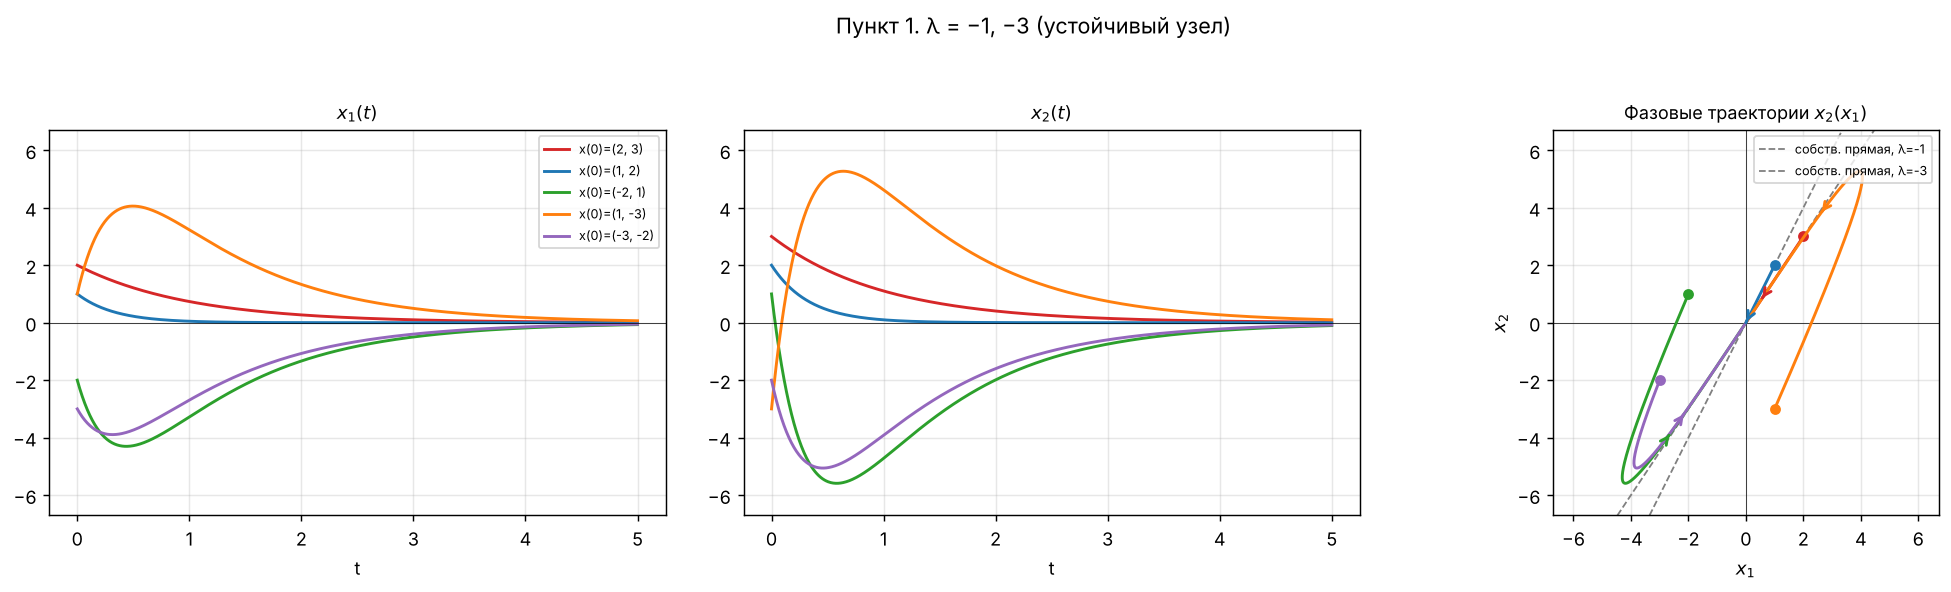
\includegraphics[width=\textwidth]{../graphics/c1_system.png}
        \caption{Пункт 1. $x_1(t)$, $x_2(t)$ и фазовые траектории (устойчивый узел)}
        \label{fig:c1}
    \end{figure}

    \subsection{Пункт 2. Неустойчивая система без двух неколлинеарных собственных векторов}
    \textbf{Выбор.} Матрица $2\times2$ не имеет двух неколлинеарных собственных векторов, если она недиагонализуема, то есть подобна жордановой клетке $J=\begin{pmatrix}\lambda&1\\0&\lambda\end{pmatrix}$. Для неустойчивости берём $\lambda=1>0$ и $A=PJP^{-1}$ (тогда $v_1$ --- собственный, $v_2$ --- обобщённый вектор):
    $$A=P\begin{pmatrix}1&1\\0&1\end{pmatrix}P^{-1}=\MatCB.$$
    $\lambda=1$ (алгебраическая кратность 2, геометрическая 1), собственный вектор $v_1$, обобщённый $v_2$: $(A-I)v_2=(2,3)^T=v_1$. Решение: $x(t)=e^{t}\bigl(x(0)+t(A-I)x(0)\bigr)$. \textbf{Тип: неустойчивый вырожденный (жорданов) узел.} Устойчивых траекторий нет, кроме $x\equiv0$: на $\Span\{v_1\}$ решение $e^{t}x(0)$ тоже растёт. Начальные условия: $v_1$, $-v_1$ (собственные), $v_2$ (обобщённый вектор), $(-2,1)^T$, $(1,-3)^T$.
    \begin{figure}[H]
        \centering
        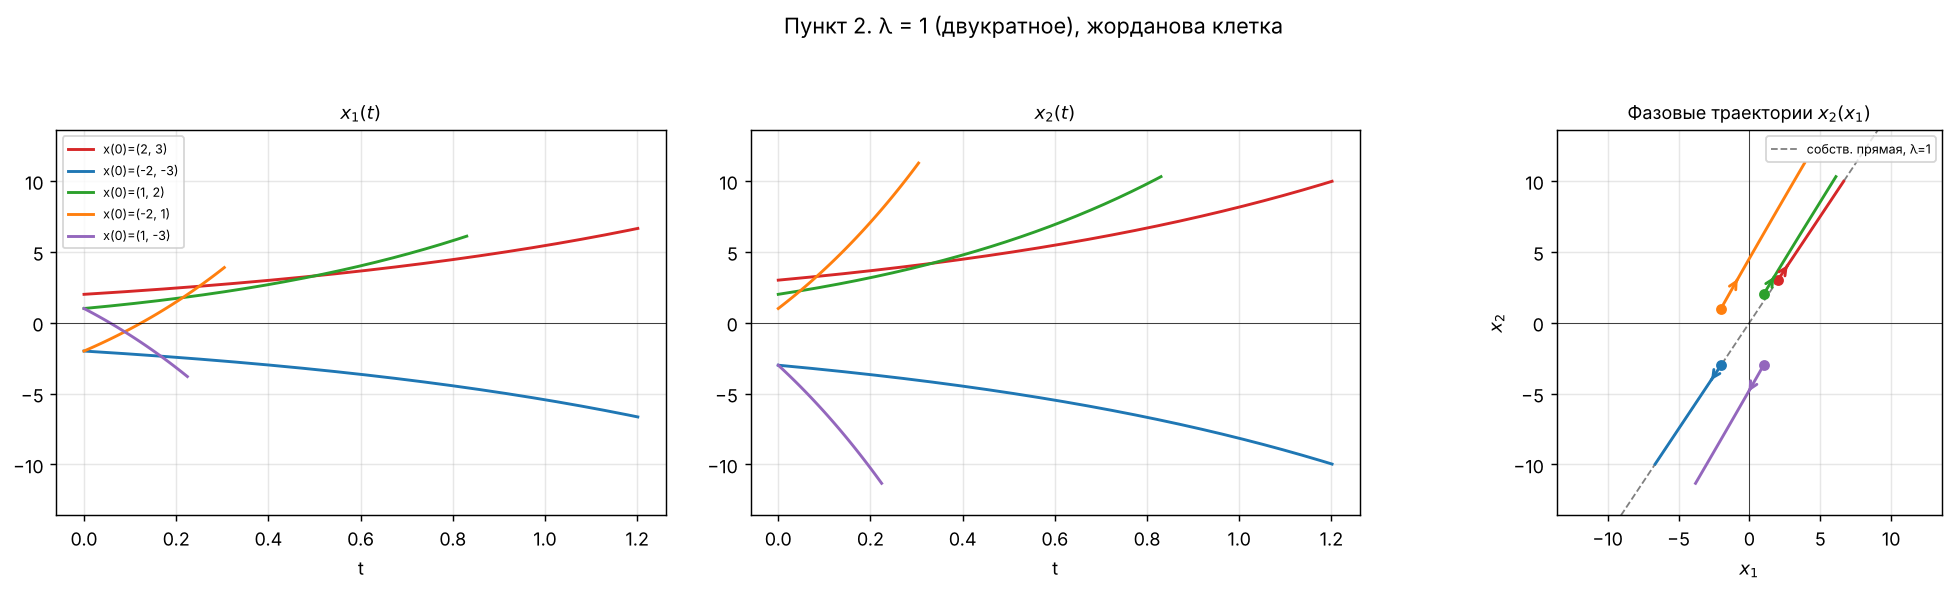
\includegraphics[width=\textwidth]{../graphics/c2_system.png}
        \caption{Пункт 2. Жорданова клетка с $\lambda=1$ (неустойчивый вырожденный узел)}
        \label{fig:c2}
    \end{figure}

    \subsection{Пункт 3. Неустойчивая система, $x(0)=v_1\Rightarrow x(t)\to0$}
    \textbf{Выбор.} Нужно, чтобы $v_1$ лежал в устойчивом подпространстве, а система в целом была неустойчива: седло. Берём $\lambda_1=-2$ ($v_1$), $\lambda_2=1$ ($v_2$):
    $$A=P\begin{pmatrix}-2&0\\0&1\end{pmatrix}P^{-1}=\MatCC.$$
    Проверка: $Av_1=(-4,-6)^T=-2v_1$, $Av_2=(1,2)^T=v_2$. Решение $x(t)=c_1e^{-2t}v_1+c_2e^{t}v_2$. \textbf{Тип: седло.} Устойчивые траектории --- только лежащие на $\Span\{v_1\}$ ($c_2=0$), все остальные уходят на бесконечность вдоль $v_2$. Они вынесены на отдельный рисунок.
    \begin{figure}[H]
        \centering
        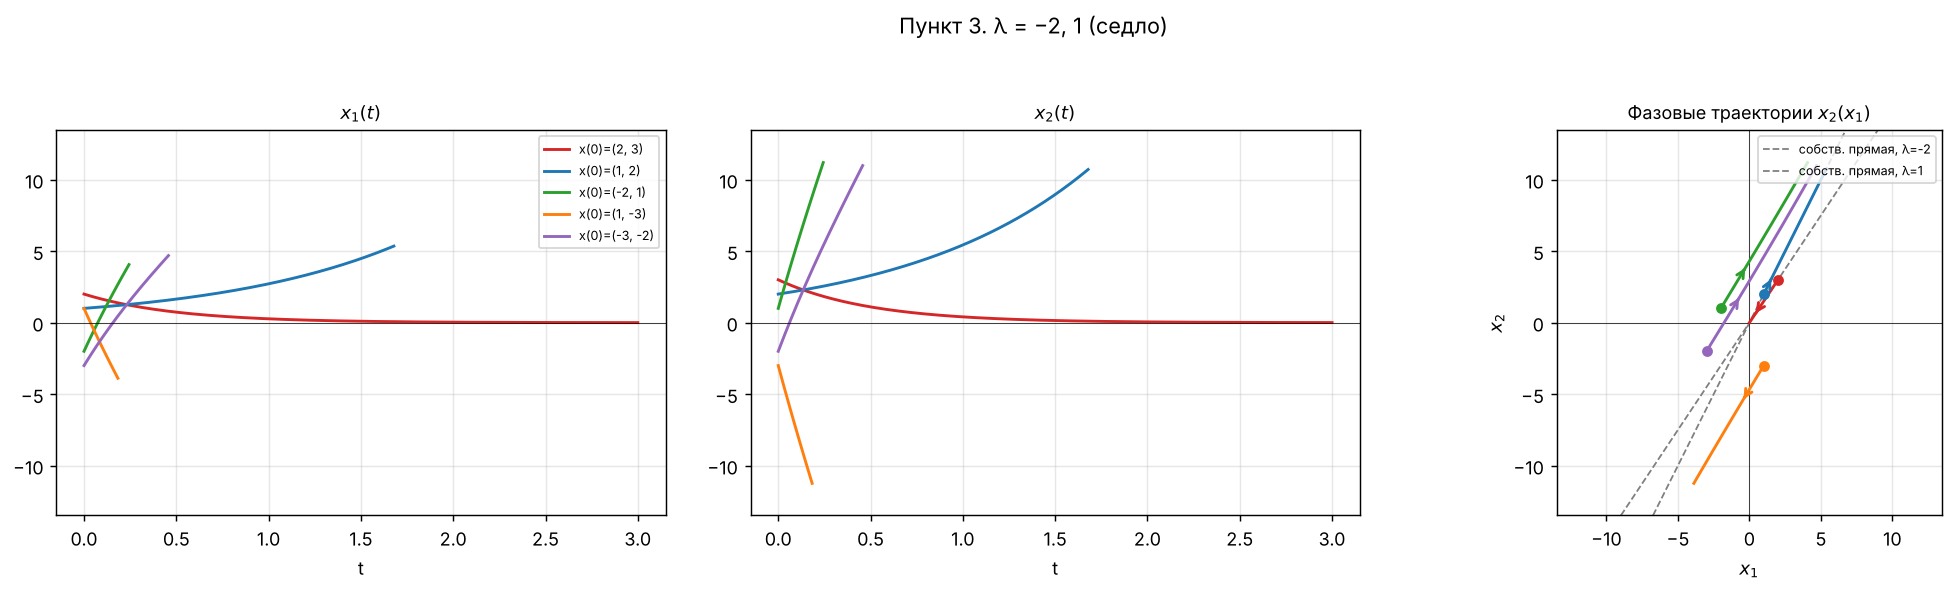
\includegraphics[width=\textwidth]{../graphics/c3_system.png}
        \caption{Пункт 3. Седло ($\lambda=-2,\,1$)}
        \label{fig:c3}
    \end{figure}
    \begin{figure}[H]
        \centering
        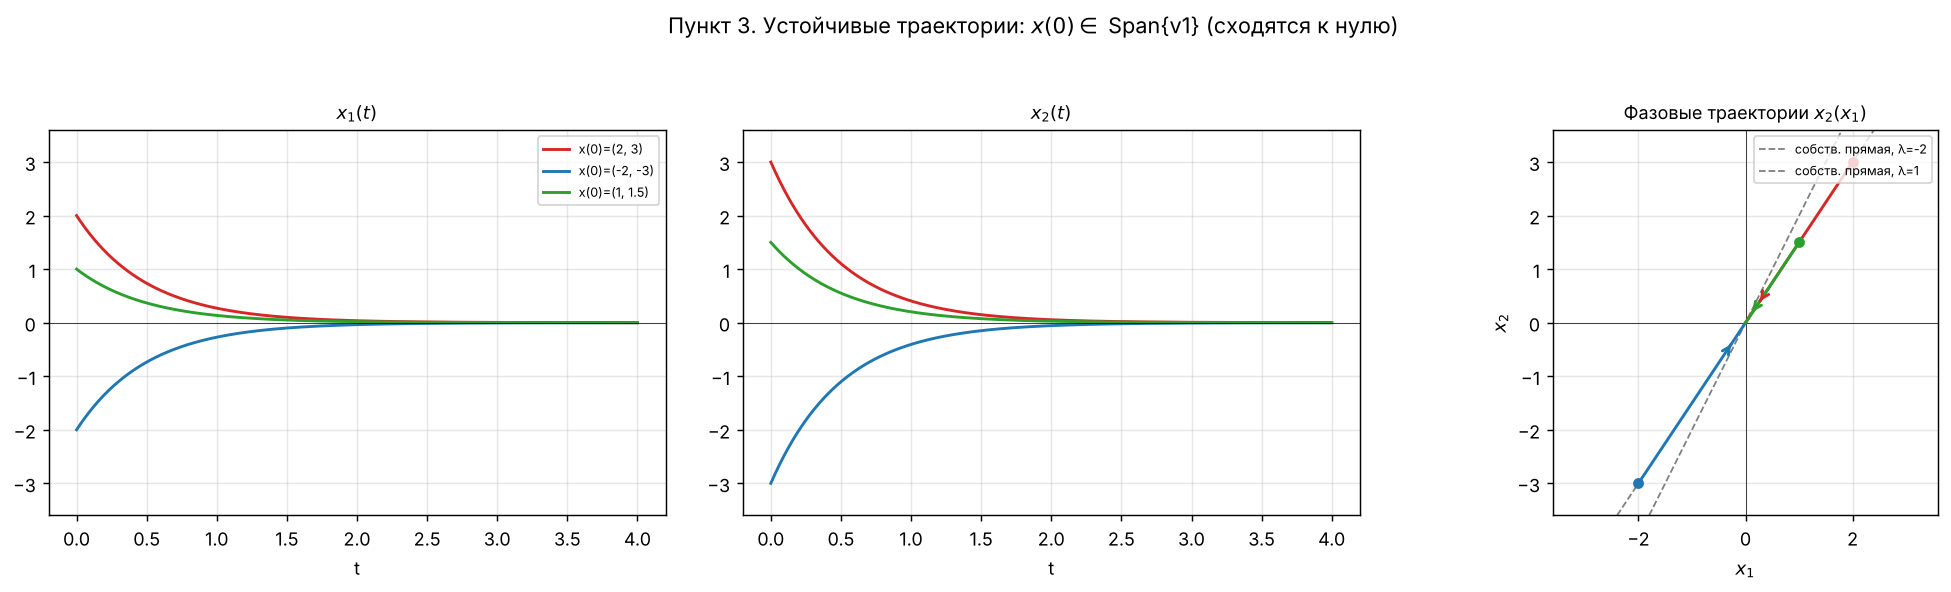
\includegraphics[width=\textwidth]{../graphics/c3_stable_only.png}
        \caption{Пункт 3. Устойчивые траектории: $x(0)\in\Span\{v_1\}$ ($x(0)=v_1$, $-v_1$, $0.5v_1$)}
        \label{fig:c3s}
    \end{figure}

    \subsection{Пункты 4--6. Комплексные собственные векторы $v_1\pm iv_2$}
    \textbf{Общая конструкция.} Пусть $A(v_1+iv_2)=(\alpha+i\beta)(v_1+iv_2)$. Приравнивая вещественные и мнимые части: $Av_1=\alpha v_1-\beta v_2$, $Av_2=\beta v_1+\alpha v_2$, то есть
    $$A=P\begin{pmatrix}\alpha&\beta\\-\beta&\alpha\end{pmatrix}P^{-1},\qquad \lambda_{1,2}=\alpha\pm i\beta,\ \ \text{векторы } v_1\pm iv_2.$$
    В координатах $y=P^{-1}x$ система превращается в $\dot y=\begin{pmatrix}\alpha&\beta\\-\beta&\alpha\end{pmatrix}y$ с решением $y(t)=e^{\alpha t}\begin{pmatrix}\cos\beta t&\sin\beta t\\-\sin\beta t&\cos\beta t\end{pmatrix}y(0)$: вращение с угловой частотой $\beta$ и множителем $e^{\alpha t}$. Устойчивость определяется знаком $\alpha$. Вещественных собственных векторов нет, поэтому начальные условия $v_1$ и $v_2$ (вещественная и мнимая части собственного вектора) --- обычные точки плоскости, а остальные три --- те же случайные.

    \textbf{Пункт 4} ($\alpha=-1$, $\beta=2$, асимптотически устойчива):
    $$A=\MatCD,\quad\lambda_{1,2}=-1\pm2i,\quad\text{векторы }v_1\pm iv_2=\begin{pmatrix}2\pm i\\3\pm2i\end{pmatrix}.$$
    \textbf{Тип портрета: устойчивый фокус} (траектории закручиваются к началу, затухая как $e^{-t}$).
    \begin{figure}[H]
        \centering
        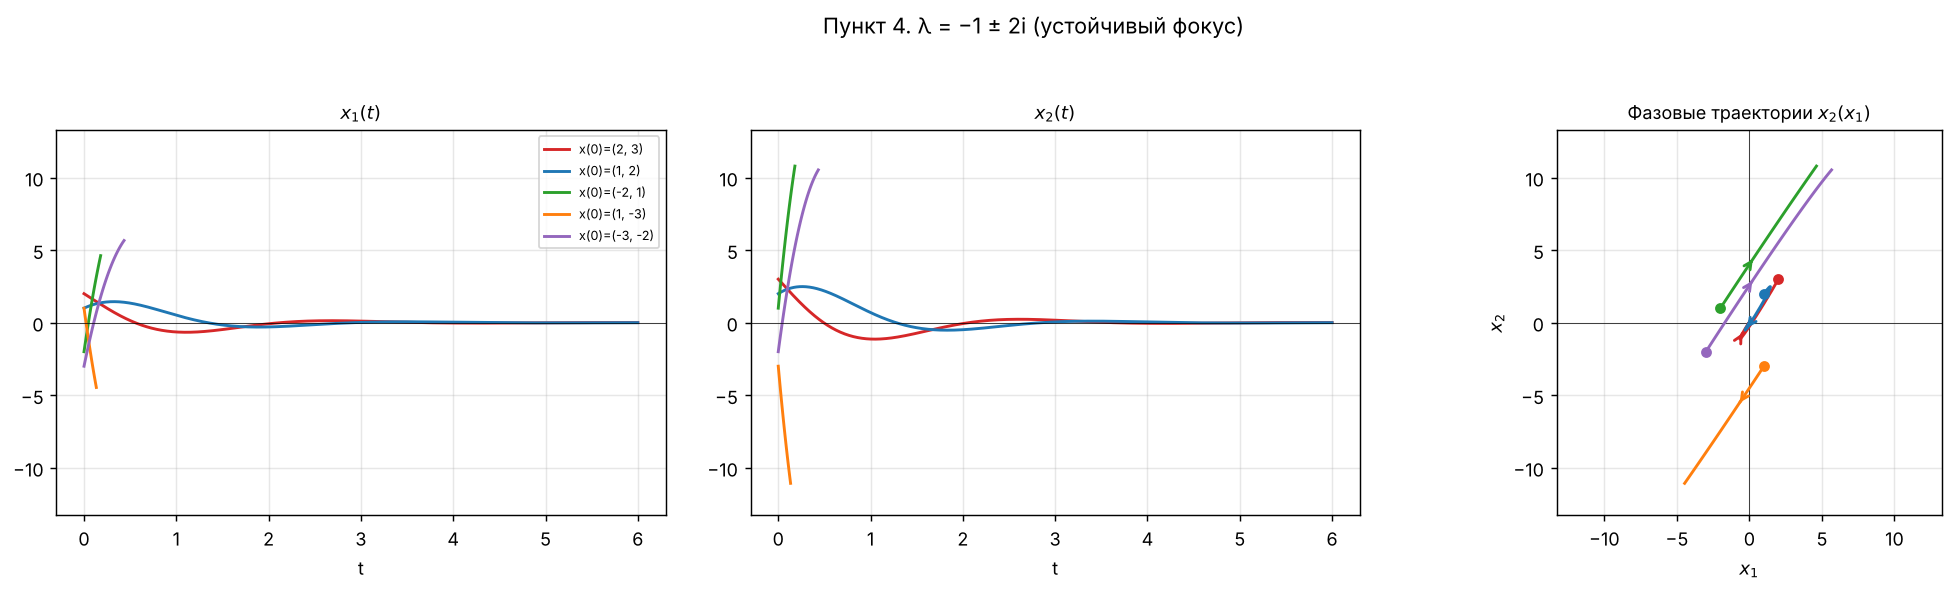
\includegraphics[width=\textwidth]{../graphics/c4_system.png}
        \caption{Пункт 4. $\lambda=-1\pm2i$ (устойчивый фокус)}
        \label{fig:c4}
    \end{figure}

    \textbf{Пункт 5} ($\alpha=1$, $\beta=2$, неустойчива, те же векторы):
    $$A=\MatCE,\quad\lambda_{1,2}=1\pm2i.$$
    \textbf{Тип: неустойчивый фокус} (раскручивающаяся спираль, $e^{t}$). Устойчивых траекторий, кроме нулевой, нет.
    \begin{figure}[H]
        \centering
        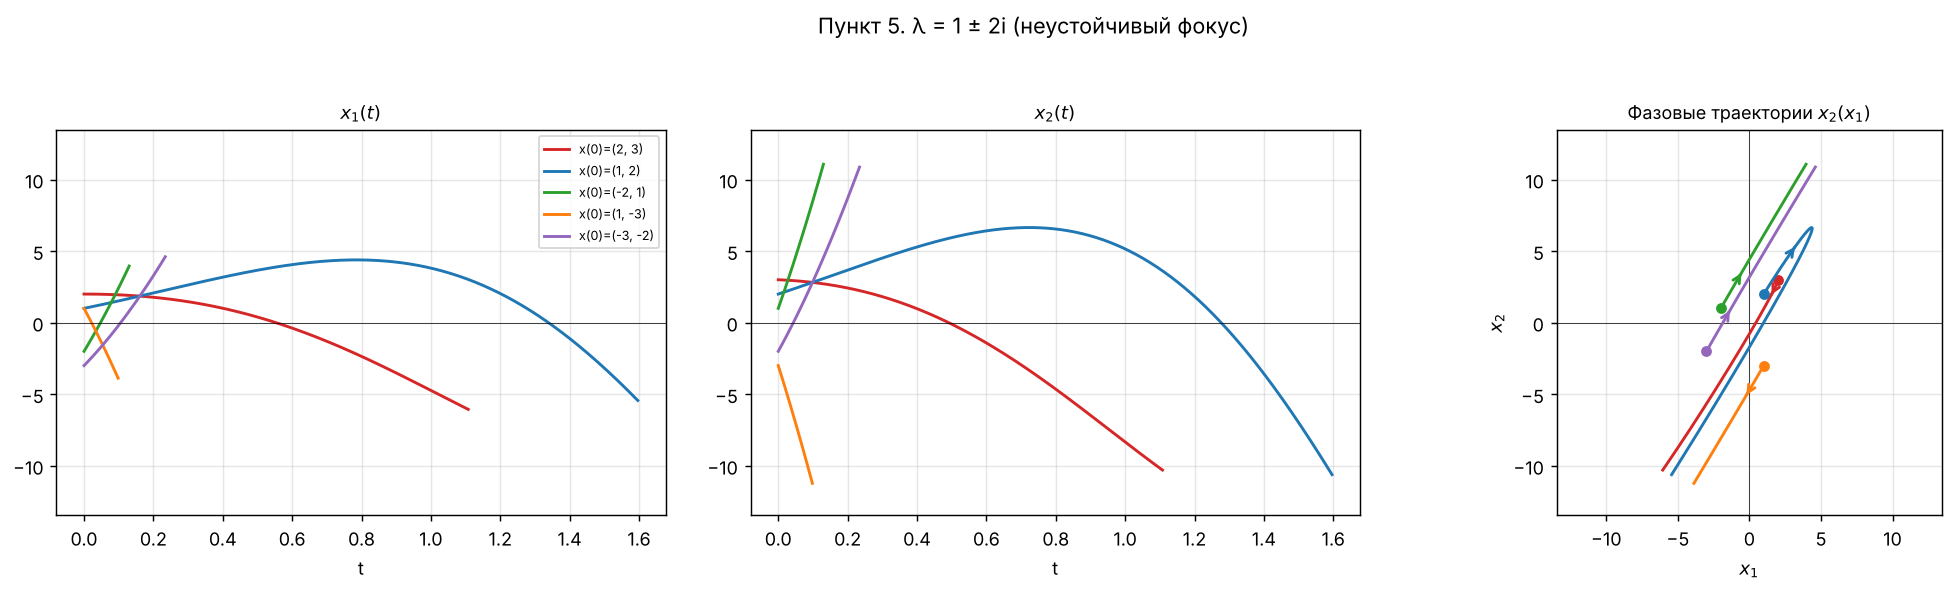
\includegraphics[width=\textwidth]{../graphics/c5_system.png}
        \caption{Пункт 5. $\lambda=1\pm2i$ (неустойчивый фокус)}
        \label{fig:c5}
    \end{figure}

    \textbf{Пункт 6} ($\alpha=0$, $\beta=2$, устойчива, но не асимптотически):
    $$A=\MatCF,\quad\lambda_{1,2}=\pm2i.$$
    \textbf{Тип: центр.} Траектории --- замкнутые эллипсы (образы окружностей при отображении $P$) с периодом $2\pi/\beta=\pi$; траектория не уходит и не стремится к нулю: расстояние до начала остаётся ограниченным, но не убывает.
    \begin{figure}[H]
        \centering
        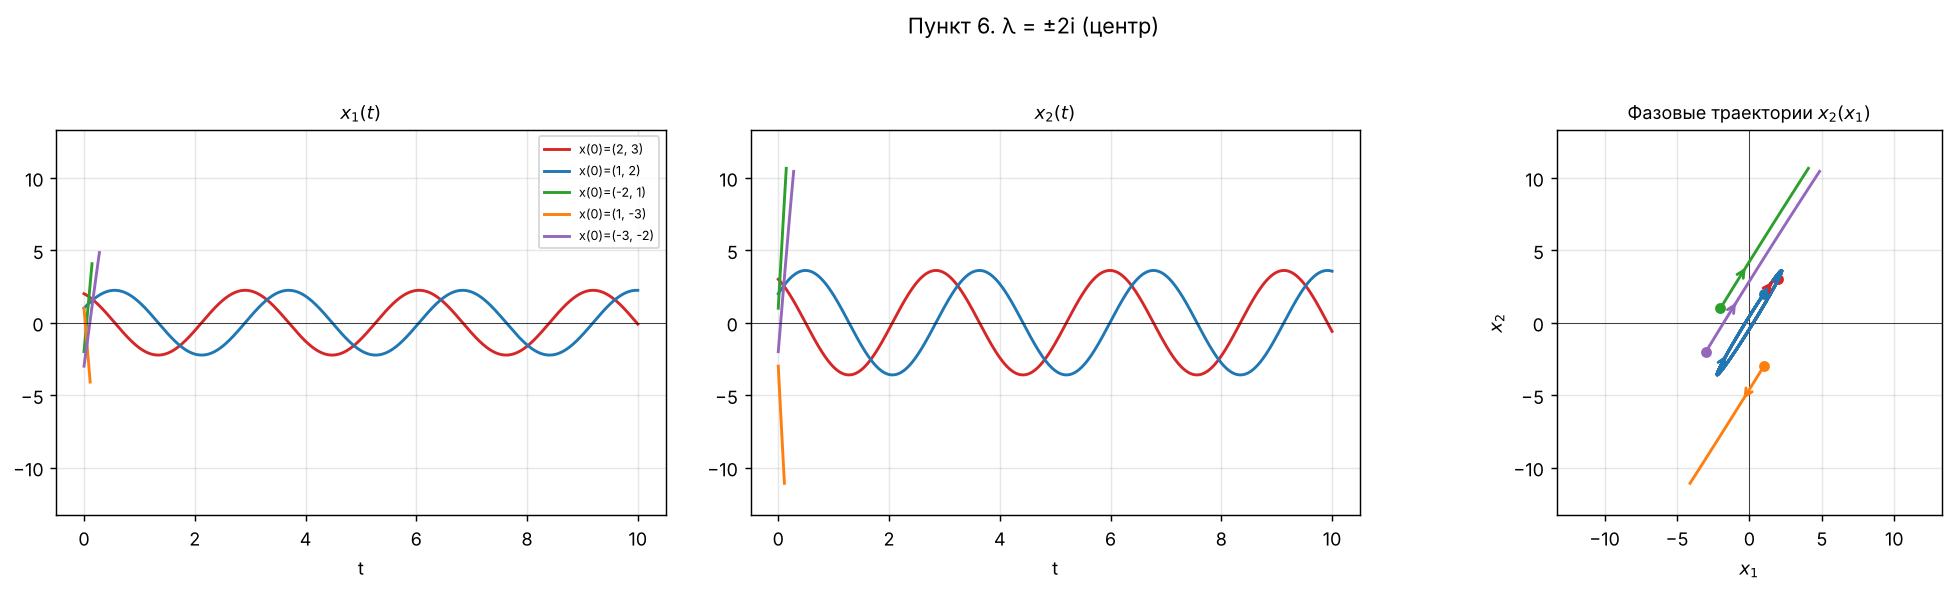
\includegraphics[width=\textwidth]{../graphics/c6_system.png}
        \caption{Пункт 6. $\lambda=\pm2i$ (центр)}
        \label{fig:c6}
    \end{figure}

    \section{Задание 2. Дискретные системы}
    \textbf{Конструкция.} Выбрана матрица $P_d=\MatPd$ ($\det P_d=1$, $P_d^{-1}=\MatPdinv$) с столбцами $p_1=(1,1)^T$, $p_2=(1,2)^T$. Все матрицы имеют вид $A=P_dMP_d^{-1}$ и потому не являются ни диагональными, ни жордановыми клетками. Матрица $M$:
    \begin{itemize}
        \item для вещественного двукратного $\lambda$ (пункты 1, 5, 6, 8, 9, 11) --- жорданова клетка $\begin{pmatrix}\lambda&1\\0&\lambda\end{pmatrix}$: собственный вектор $p_1$, обобщённый $p_2$ ($(A-\lambda I)p_2=p_1$); решение $x(k)=P_d\begin{pmatrix}\lambda^k&k\lambda^{k-1}\\0&\lambda^k\end{pmatrix}P_d^{-1}x(0)$;
        \item для комплексной пары $\lambda=re^{\pm i\varphi}$ (пункты 2, 3, 4, 7, 10) --- блок $r\begin{pmatrix}\cos\varphi&\sin\varphi\\-\sin\varphi&\cos\varphi\end{pmatrix}$: собственные векторы $p_1\pm ip_2=(1\pm i,\,1\pm2i)^T$ (для $+$ --- число $re^{i\varphi}$); в координатах $y=P_d^{-1}x$ система поворачивает на угол $\varphi$ и умножает на $r$ за один шаг;
        \item для $\lambda=0$ (пункт 12) --- нильпотентная клетка $\begin{pmatrix}0&1\\0&0\end{pmatrix}$, $A^2=0$.
    \end{itemize}
    Константы: $c=0.8$ ($0<c<1$), $d=1.2$ ($d>1$). Начальные условия: $(2,1)^T$, $(-1,2)^T$, $(1.5,-1)^T$, $k=0,\dots,25$. На каждом рисунке: $x_1(k)$, $x_2(k)$, фазовые кривые $x_2(x_1)$ (квадратик --- начальная точка) и собственные числа на комплексной плоскости (пунктир --- единичная окружность).

    \begin{table}[H]
        \centering
        \caption{Задание 2: собственные числа и устойчивость}
        \label{tab:disc}
        \begin{tabular}{@{}clcl@{}}
            \toprule
            № & $\lambda_{1,2}$ & $|\lambda|$ & Устойчивость \\
            \midrule
            1 & $-1$ (двукратное, жорданова) & 1 & неустойчива \\
            2 & $-\frac1{\sqrt2}\pm\frac i{\sqrt2}$ & 1 & устойчива, не асимптотически \\
            3 & $\pm i$ & 1 & устойчива, не асимптотически \\
            4 & $\frac1{\sqrt2}\pm\frac i{\sqrt2}$ & 1 & устойчива, не асимптотически \\
            5 & $1$ (двукратное, жорданова) & 1 & неустойчива \\
            6 & $-0.8$ (двукратное) & 0.8 & асимптотически устойчива \\
            7 & $\pm0.8i$ & 0.8 & асимптотически устойчива \\
            8 & $0.8$ (двукратное) & 0.8 & асимптотически устойчива \\
            9 & $-1.2$ (двукратное) & 1.2 & неустойчива \\
            10 & $\pm1.2i$ & 1.2 & неустойчива \\
            11 & $1.2$ (двукратное) & 1.2 & неустойчива \\
            12 & $0$ (двукратное) & 0 & асимптотически устойчива (за 2 шага) \\
            \bottomrule
        \end{tabular}
    \end{table}
    \begin{figure}[H]
        \centering
        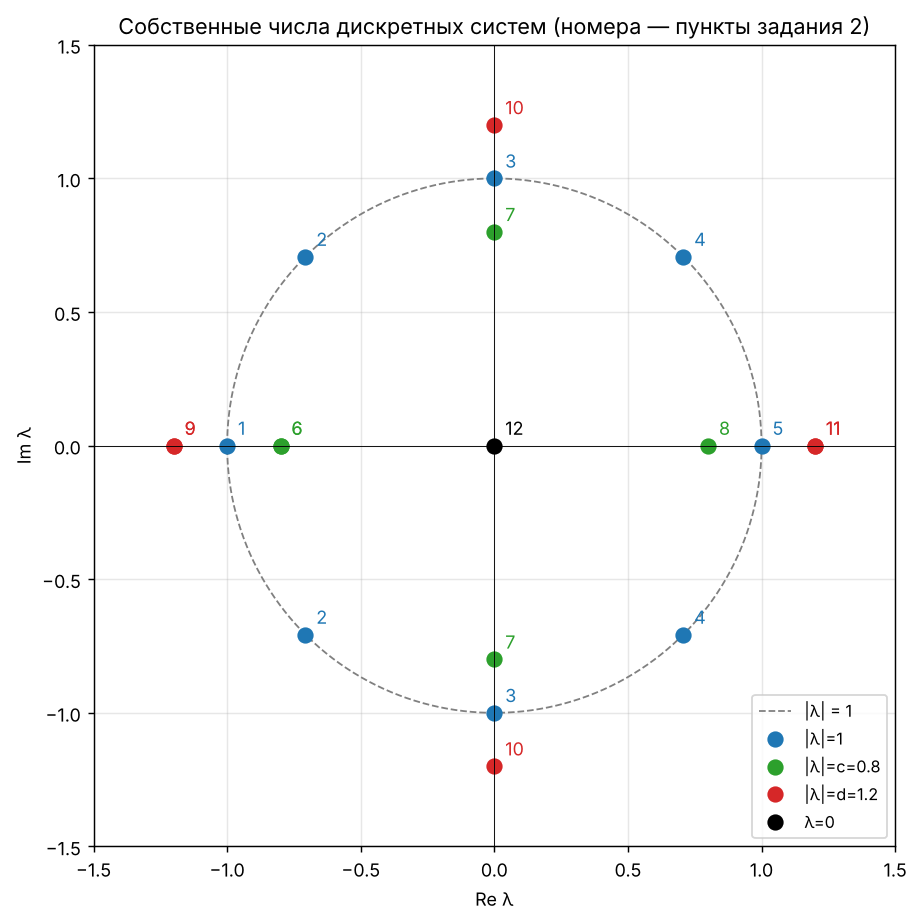
\includegraphics[width=0.65\textwidth]{../graphics/d_eigenvalues.png}
        \caption{Собственные числа всех систем задания 2 на комплексной плоскости (номера --- пункты)}
        \label{fig:deig}
    \end{figure}

    \subsection{Пункт 1. $\lambda_{1,2}=-1$}
    $A=\MatDA$ (подобна $\begin{pmatrix}-1&1\\0&-1\end{pmatrix}$). Собственный вектор $p_1=(1,1)^T$, обобщённый $p_2=(1,2)^T$. $A^k$ содержит множитель $k(-1)^{k-1}$: любые решения, не лежащие на $\Span\{p_1\}$, растут линейно по $k$ с чередованием знака. \textbf{Неустойчива} (жорданова клетка на границе $|\lambda|=1$). Устойчивые (ограниченные) траектории: $x(0)\in\Span\{p_1\}$, $x(k)=(-1)^kx(0)$ (рисунок~\ref{fig:d1s}).
    \begin{figure}[H]
        \centering
        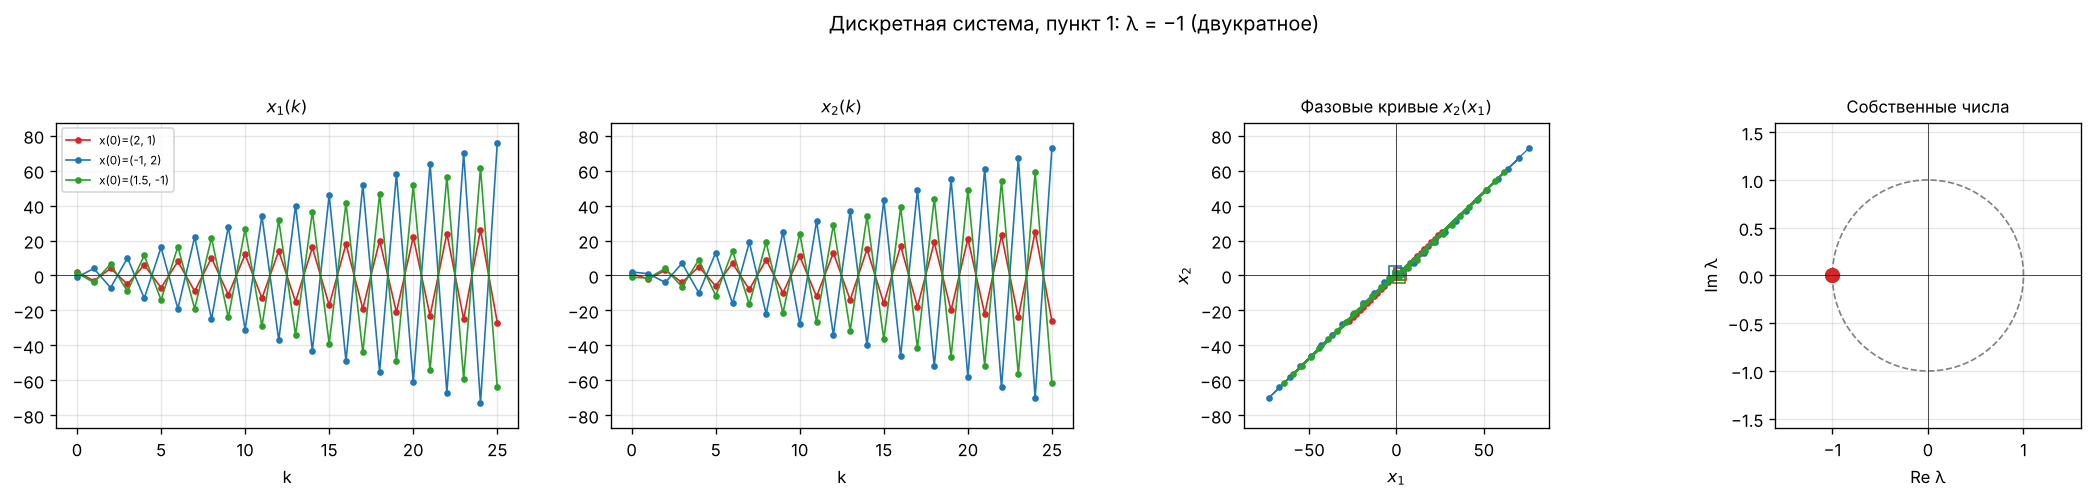
\includegraphics[width=\textwidth]{../graphics/d1_system.png}
        \caption{Пункт 1. $\lambda=-1$ (жорданова структура)}
        \label{fig:d1}
    \end{figure}
    \begin{figure}[H]
        \centering
        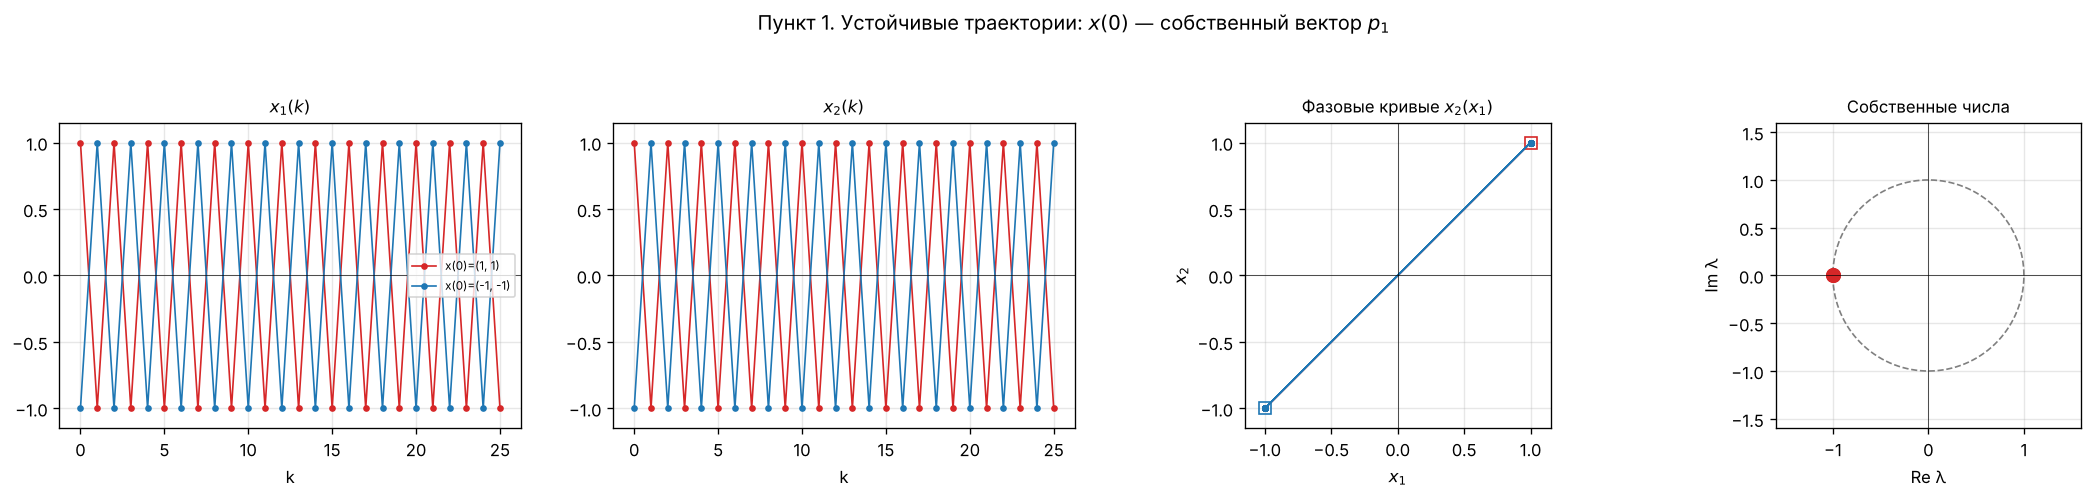
\includegraphics[width=\textwidth]{../graphics/d1_stable_only.png}
        \caption{Пункт 1. Устойчивые траектории $x(0)=\pm p_1$: $x(k)=(-1)^kx(0)$}
        \label{fig:d1s}
    \end{figure}

    \subsection{Пункт 2. $\lambda_{1,2}=-\frac1{\sqrt2}\pm\frac1{\sqrt2}i$}
    $A=\MatDB$. Собственные числа $e^{\pm i\,3\pi/4}$, $|\lambda|=1$, векторы $p_1\pm ip_2$. За шаг поворот на $135^\circ$ (в координатах $y=P_d^{-1}x$), траектория периодическая с периодом 8 шагов и лежит на эллипсе. \textbf{Устойчива, но не асимптотически} (колебания не затухают и не растут).
    \begin{figure}[H]
        \centering
        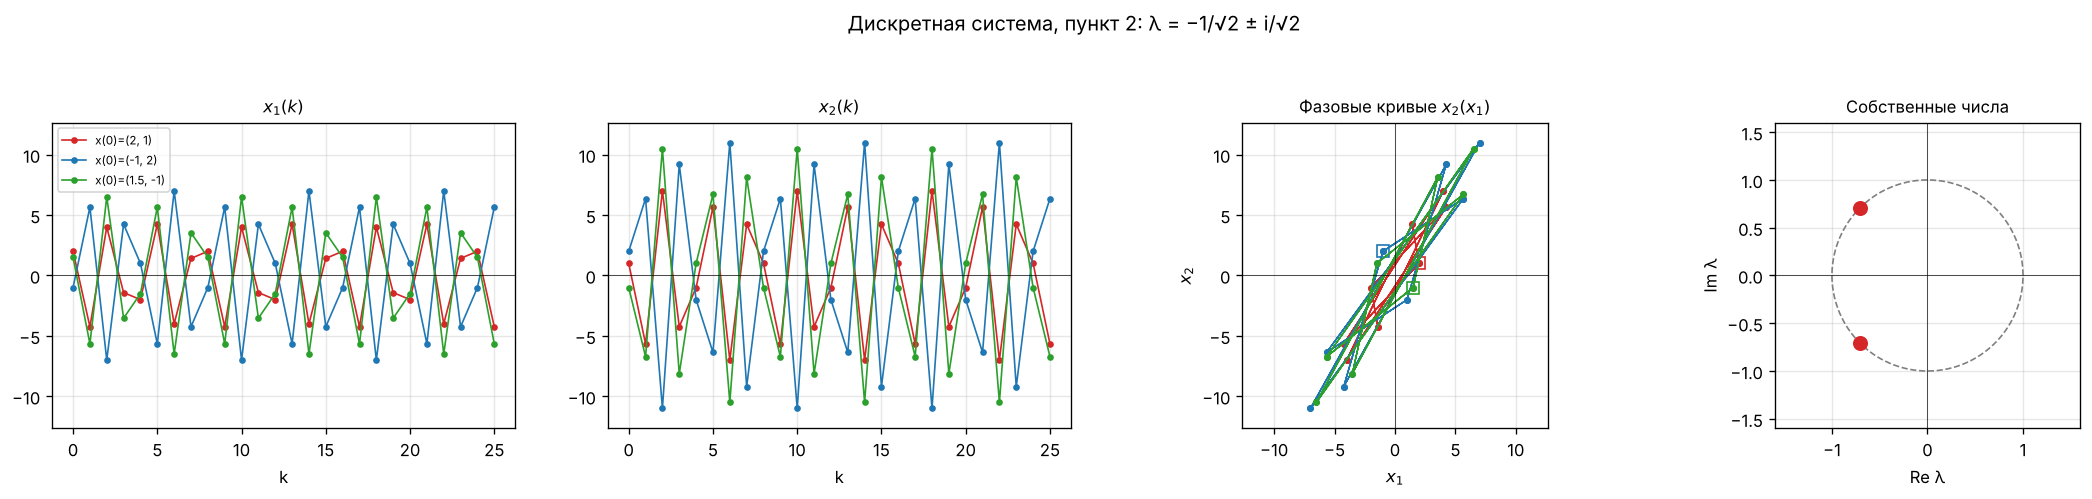
\includegraphics[width=\textwidth]{../graphics/d2_system.png}
        \caption{Пункт 2}
        \label{fig:d2}
    \end{figure}

    \subsection{Пункт 3. $\lambda_{1,2}=\pm i$}
    $A=\MatDC$. $\lambda=e^{\pm i\pi/2}$, векторы $(1\pm i,\,1\pm2i)^T$. Поворот на $90^\circ$ за шаг, $A^4=I$, период 4. \textbf{Устойчива, не асимптотически.}
    \begin{figure}[H]
        \centering
        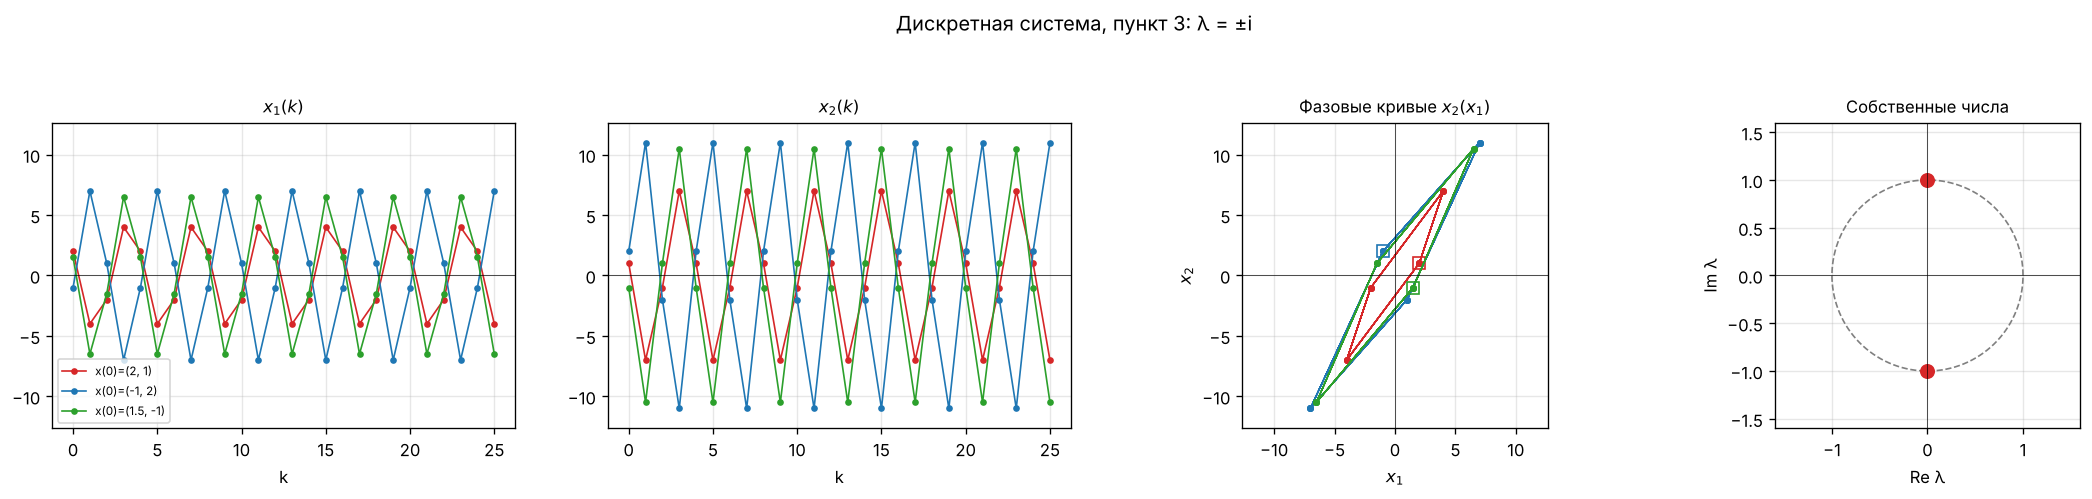
\includegraphics[width=\textwidth]{../graphics/d3_system.png}
        \caption{Пункт 3}
        \label{fig:d3}
    \end{figure}

    \subsection{Пункт 4. $\lambda_{1,2}=\frac1{\sqrt2}\pm\frac1{\sqrt2}i$}
    $A=\MatDD$. $\lambda=e^{\pm i\pi/4}$, поворот на $45^\circ$ за шаг, период 8. \textbf{Устойчива, не асимптотически.} В отличие от пункта 2 вращение медленнее: $45^\circ$ за шаг вместо $135^\circ$.
    \begin{figure}[H]
        \centering
        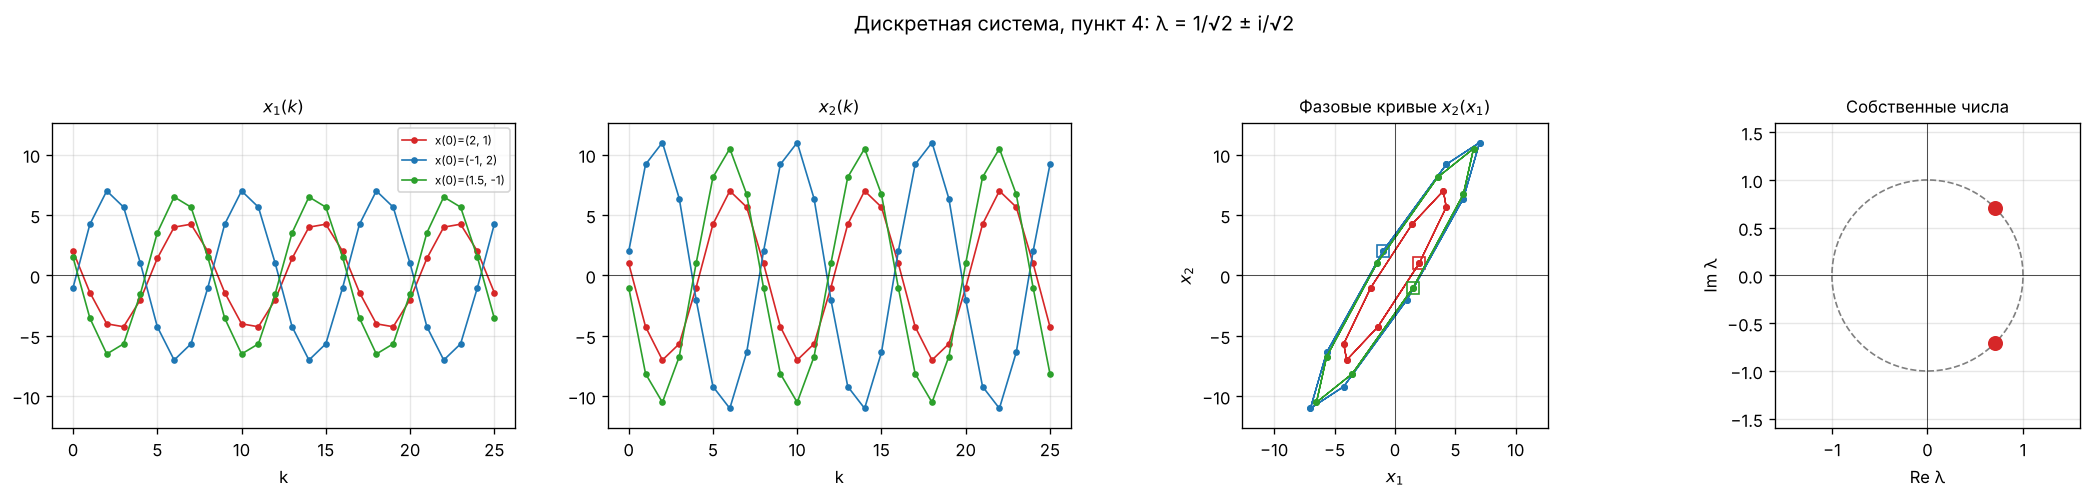
\includegraphics[width=\textwidth]{../graphics/d4_system.png}
        \caption{Пункт 4}
        \label{fig:d4}
    \end{figure}

    \subsection{Пункт 5. $\lambda_{1,2}=1$}
    $A=\MatDE$. Собственный вектор $p_1$, обобщённый $p_2$. $x(k)=x(0)+k\,(A-I)x(0)$: линейный дрейф вдоль $p_1$. \textbf{Неустойчива.} Устойчивые траектории --- неподвижные точки $x(0)\in\Span\{p_1\}$ (рисунок~\ref{fig:d5s}).
    \begin{figure}[H]
        \centering
        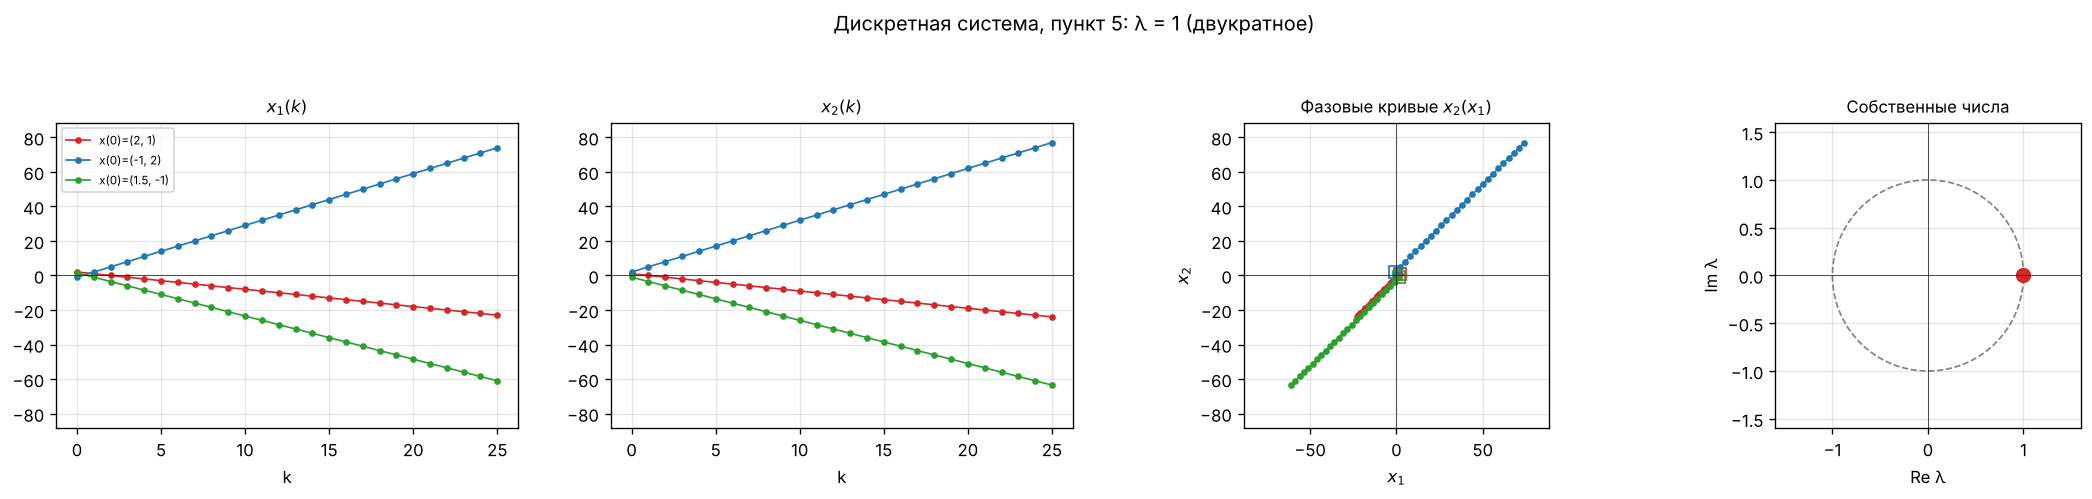
\includegraphics[width=\textwidth]{../graphics/d5_system.png}
        \caption{Пункт 5. $\lambda=1$ (дрейф вдоль $p_1$)}
        \label{fig:d5}
    \end{figure}
    \begin{figure}[H]
        \centering
        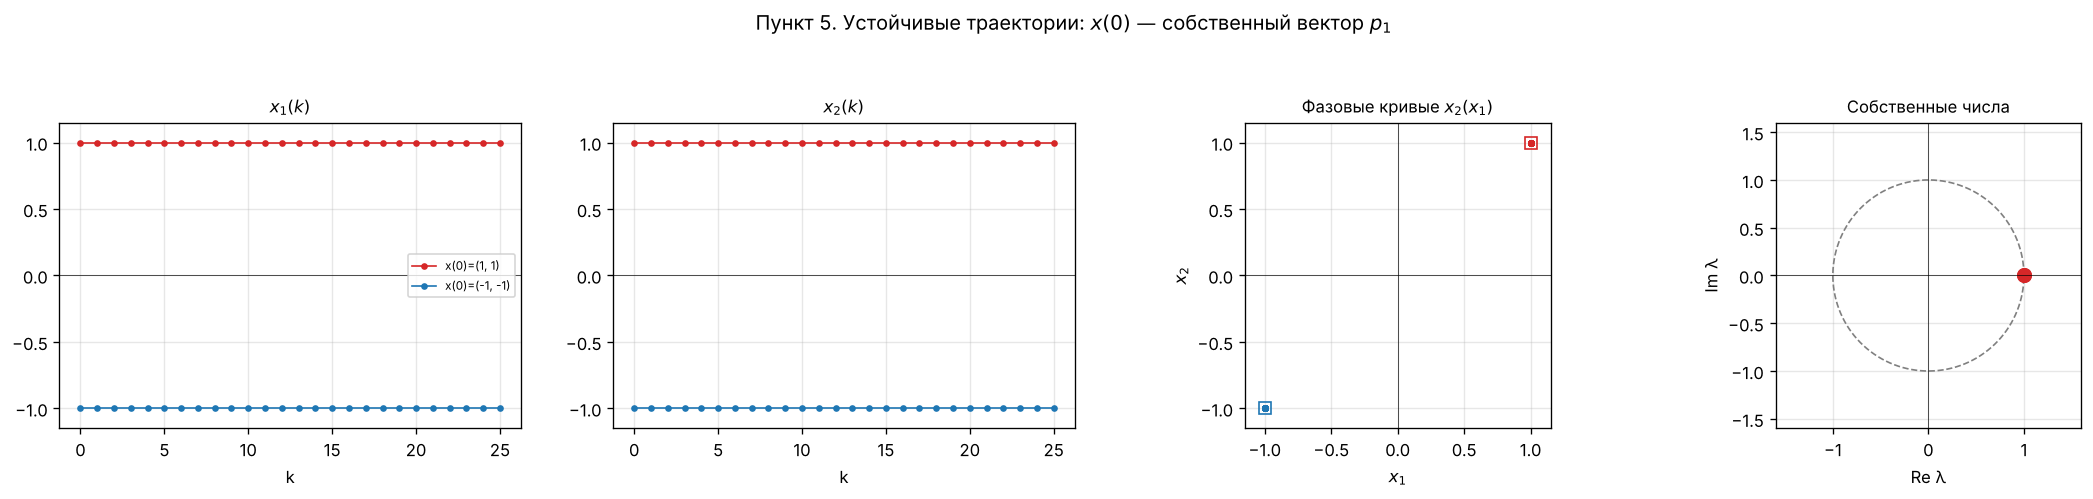
\includegraphics[width=\textwidth]{../graphics/d5_stable_only.png}
        \caption{Пункт 5. Устойчивые траектории $x(0)=\pm p_1$ --- неподвижные точки}
        \label{fig:d5s}
    \end{figure}

    \subsection{Пункты 6--8. Собственные числа пунктов 1, 3, 5, умноженные на $c=0.8$}
    \textbf{Пункт 6} ($\lambda=-0.8$): $A=\MatDF$. $x(k)\sim(-0.8)^k(1+\mathrm{const}\cdot k)$: знак чередуется, амплитуда затухает после небольшого горба (из-за жордановой клетки). \textbf{Асимптотически устойчива.}
    \begin{figure}[H]
        \centering
        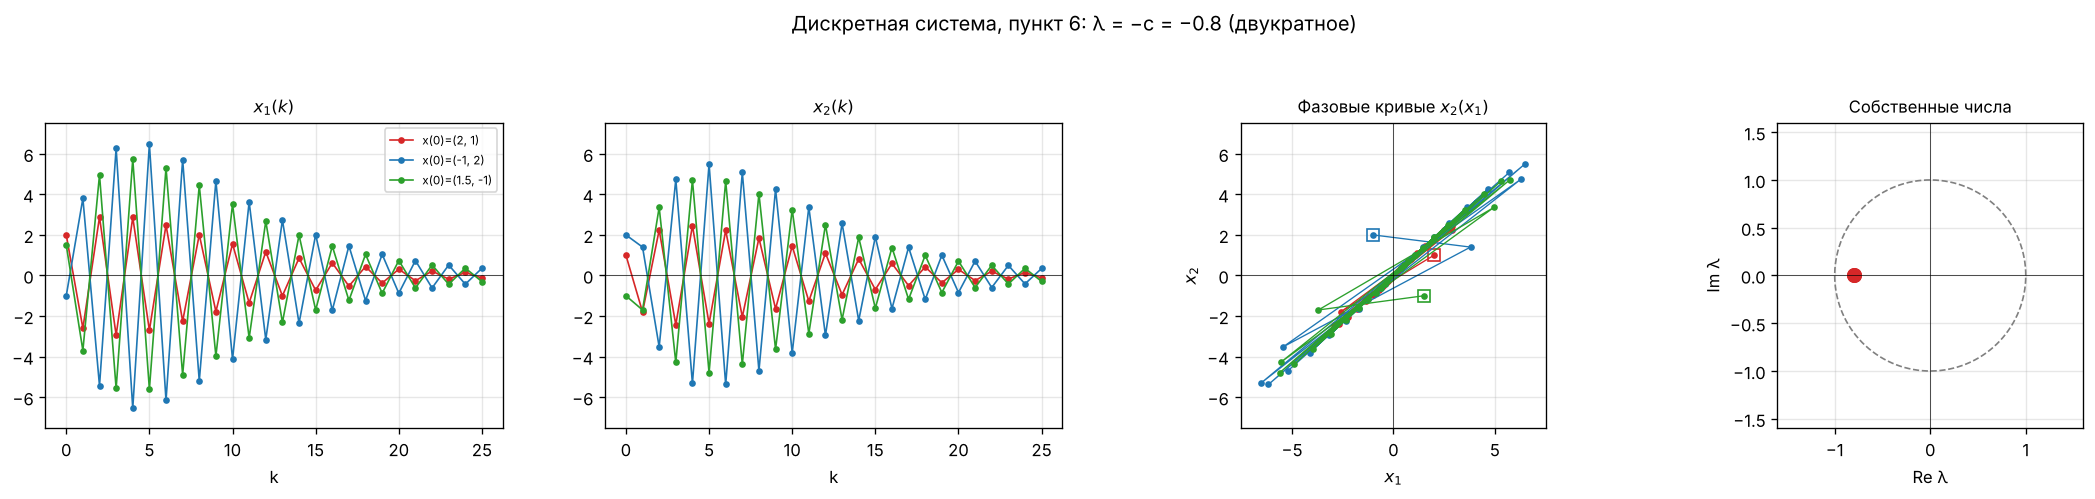
\includegraphics[width=\textwidth]{../graphics/d6_system.png}
        \caption{Пункт 6}
        \label{fig:d6}
    \end{figure}
    \textbf{Пункт 7} ($\lambda=\pm0.8i$): $A=\MatDG$. Поворот на $90^\circ$ и сжатие в $0.8$ раза за шаг: спираль к нулю. \textbf{Асимптотически устойчива} (устойчивый фокус).
    \begin{figure}[H]
        \centering
        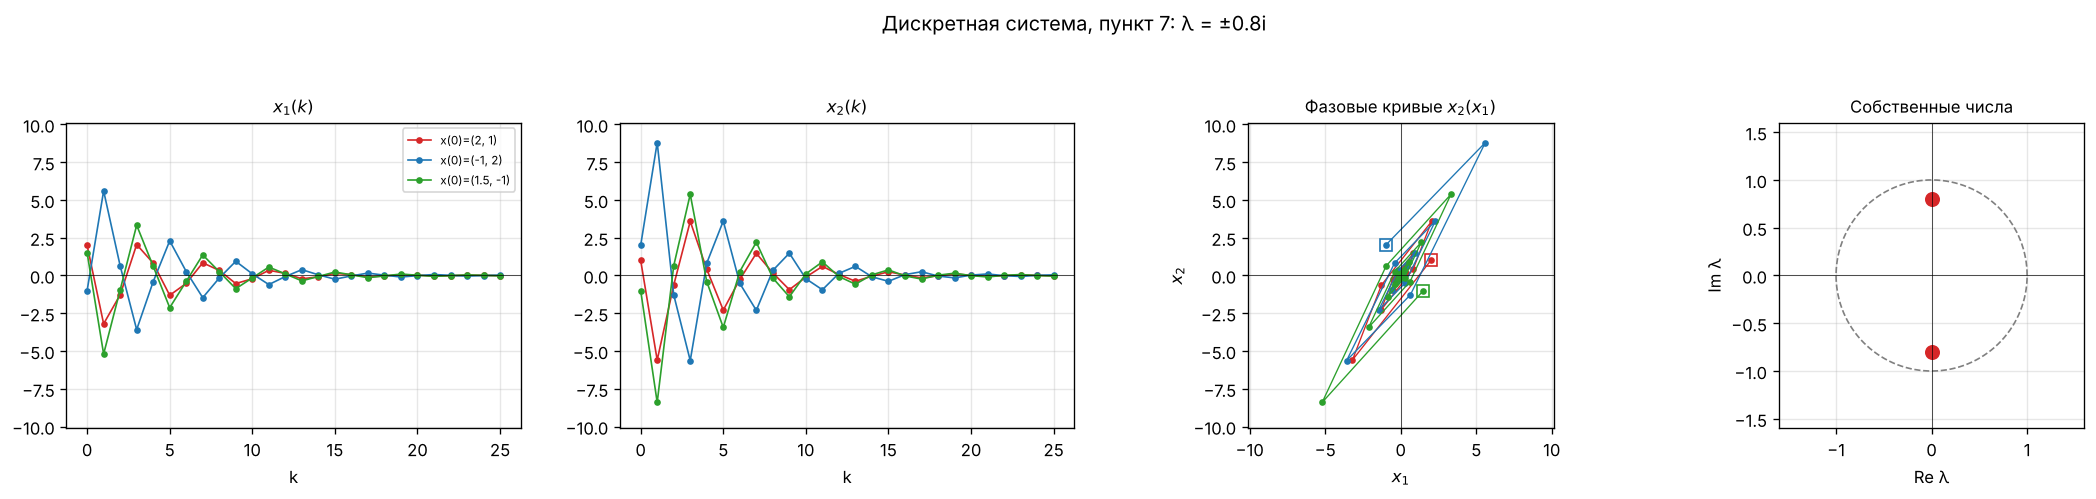
\includegraphics[width=\textwidth]{../graphics/d7_system.png}
        \caption{Пункт 7}
        \label{fig:d7}
    \end{figure}
    \textbf{Пункт 8} ($\lambda=0.8$): $A=\MatDH$. Монотонное затухание без смены знака (после возможного горба). \textbf{Асимптотически устойчива} (узел).
    \begin{figure}[H]
        \centering
        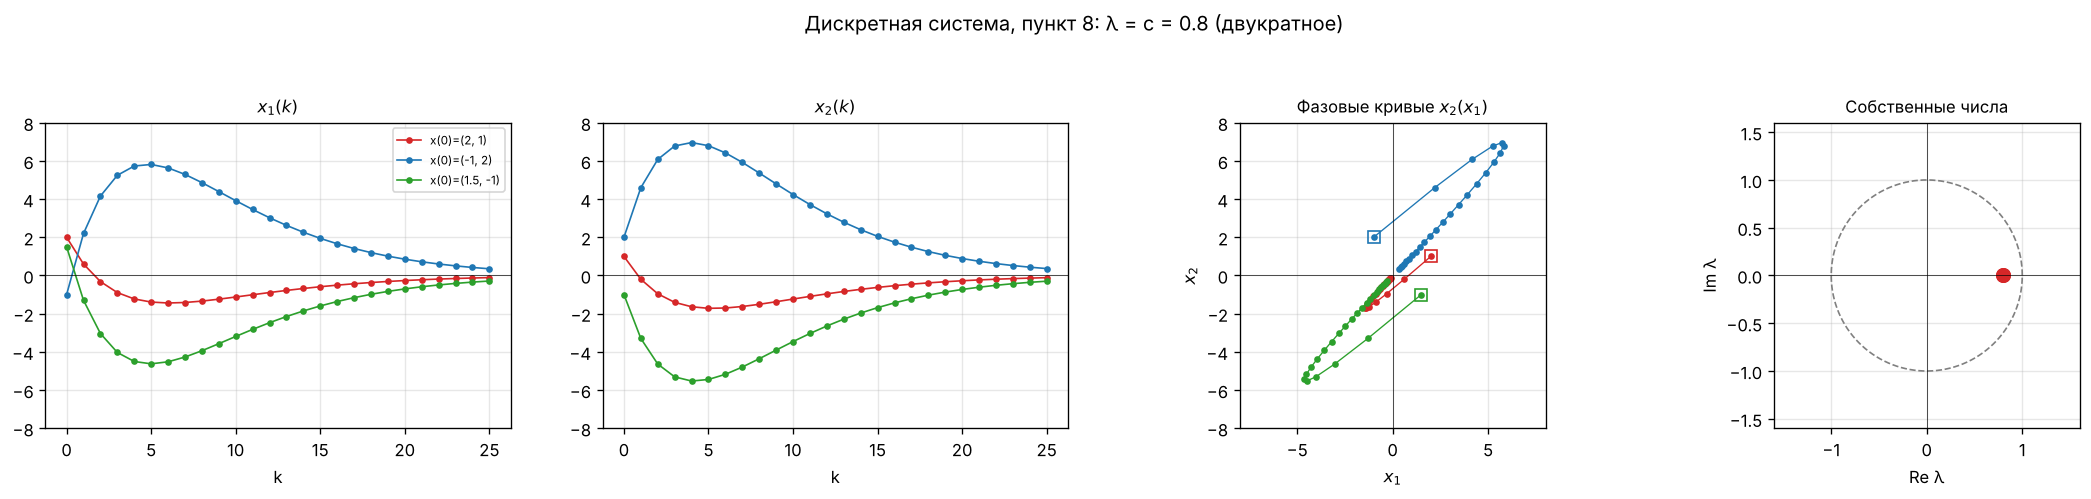
\includegraphics[width=\textwidth]{../graphics/d8_system.png}
        \caption{Пункт 8}
        \label{fig:d8}
    \end{figure}

    \subsection{Пункты 9--11. Собственные числа пунктов 1, 3, 5, умноженные на $d=1.2$}
    \textbf{Пункт 9} ($\lambda=-1.2$): $A=\MatDI$. Знакопеременный рост по закону $\sim1.2^k k$. \textbf{Неустойчива.} \textbf{Пункт 10} ($\lambda=\pm1.2i$): $A=\MatDJ$. Поворот на $90^\circ$ и растяжение в $1.2$ раза: раскручивающаяся спираль. \textbf{Неустойчива.} \textbf{Пункт 11} ($\lambda=1.2$): $A=\MatDK$. Монотонный рост. \textbf{Неустойчива.} Устойчивых траекторий (кроме нулевой) нет: все $|\lambda|>1$.
    \begin{figure}[H]
        \centering
        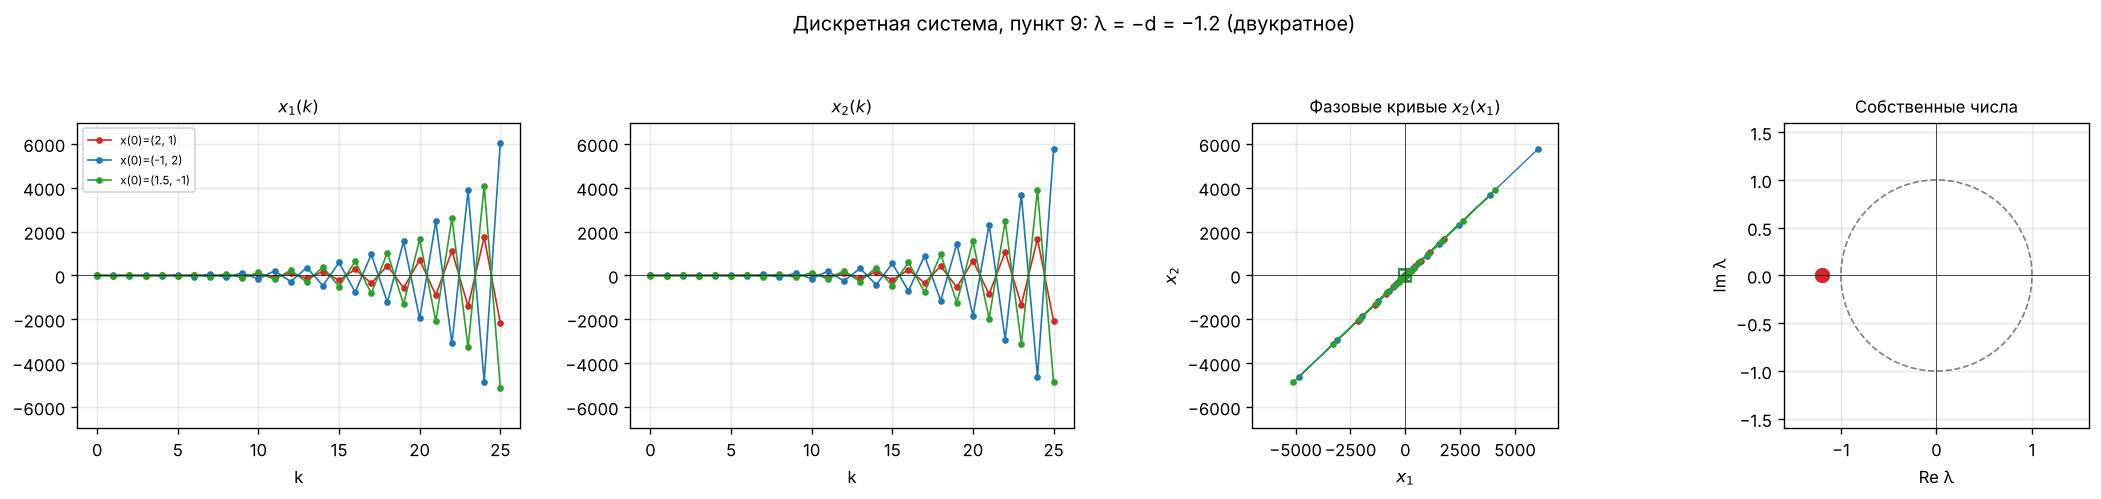
\includegraphics[width=\textwidth]{../graphics/d9_system.png}
        \caption{Пункт 9}
        \label{fig:d9}
    \end{figure}
    \begin{figure}[H]
        \centering
        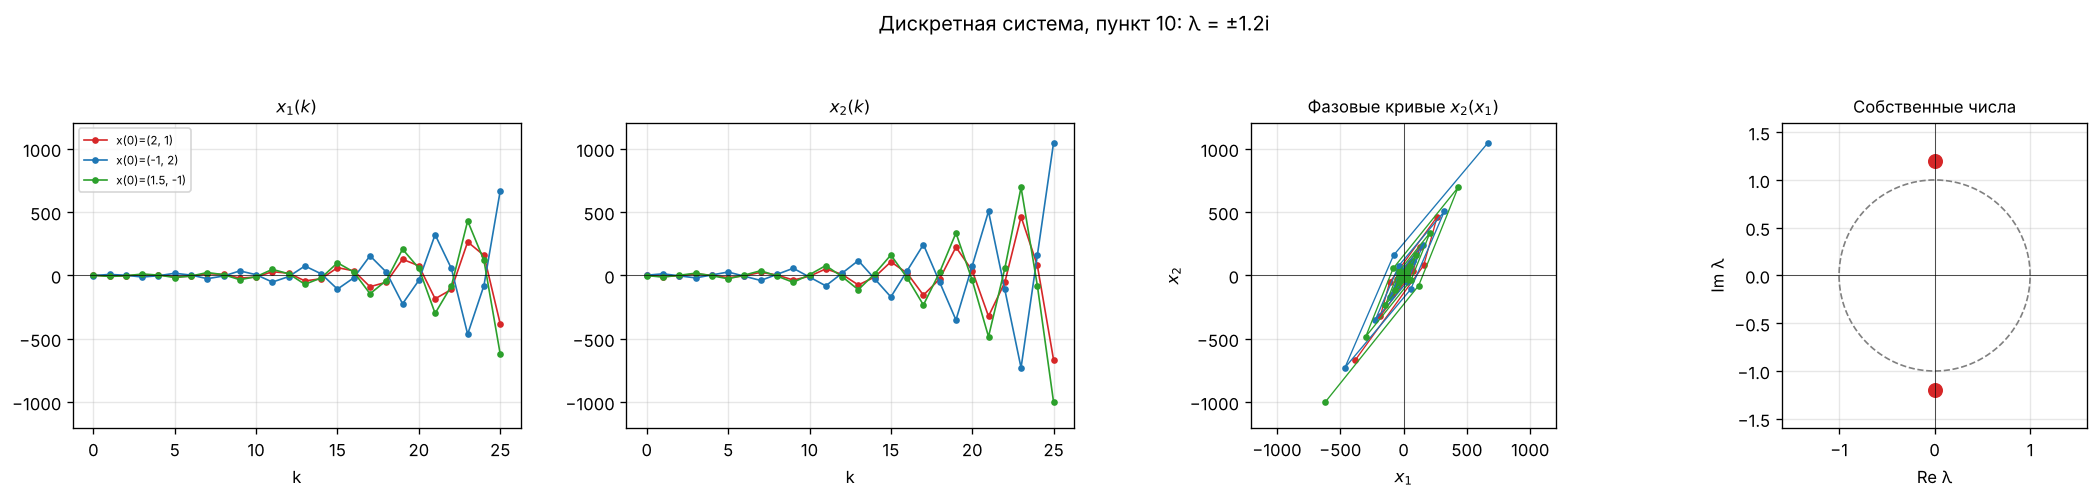
\includegraphics[width=\textwidth]{../graphics/d10_system.png}
        \caption{Пункт 10}
        \label{fig:d10}
    \end{figure}
    \begin{figure}[H]
        \centering
        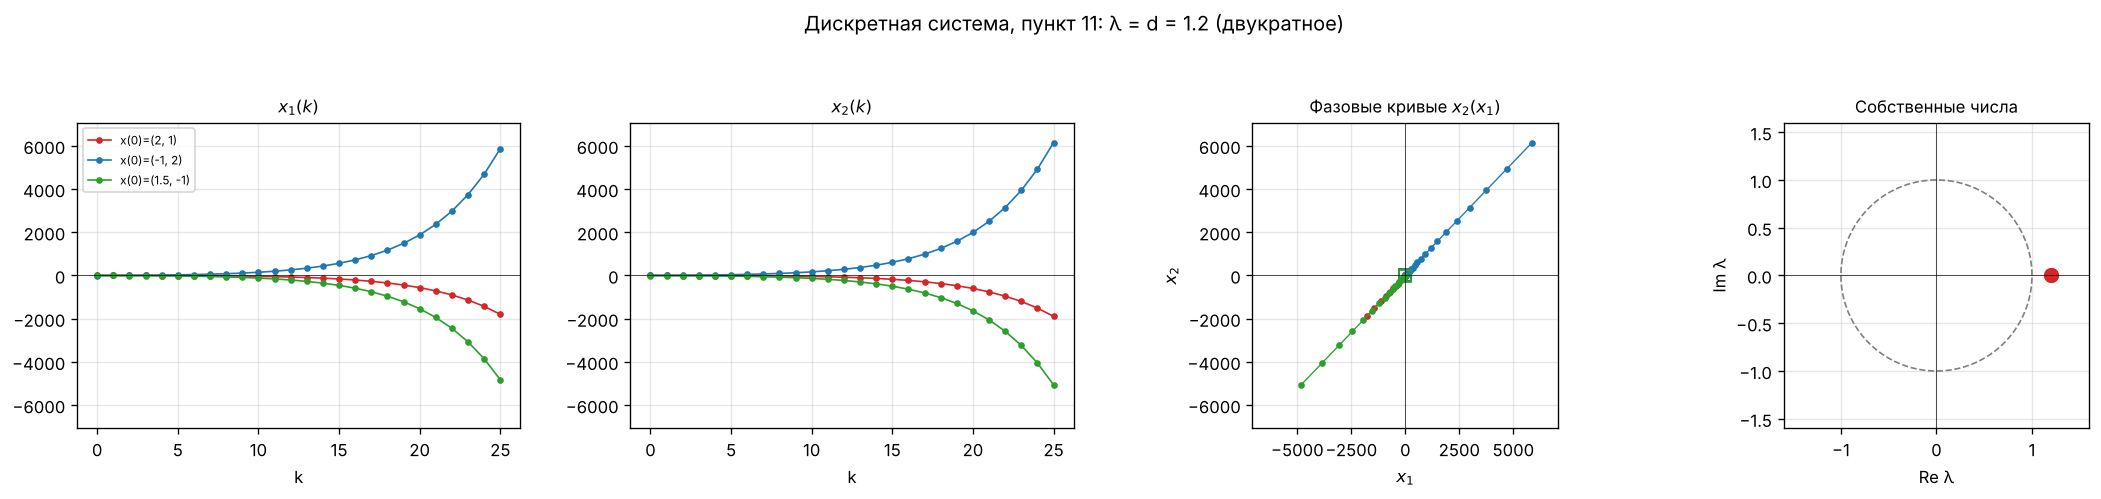
\includegraphics[width=\textwidth]{../graphics/d11_system.png}
        \caption{Пункт 11}
        \label{fig:d11}
    \end{figure}

    \subsection{Пункт 12. $\lambda_{1,2}=0$}
    $A=\MatDL$ (нильпотентная матрица, $A\neq0$, $A^2=0$), собственный вектор $p_1$, обобщённый $p_2$ ($Ap_2=p_1$). $x(0)\mapsto x(1)=Ax(0)\in\Span\{p_1\}\mapsto x(2)=A^2x(0)=0$: \textbf{сходимость к нулю за два шага} при любом $x(0)$. Асимптотически устойчива.
    \begin{figure}[H]
        \centering
        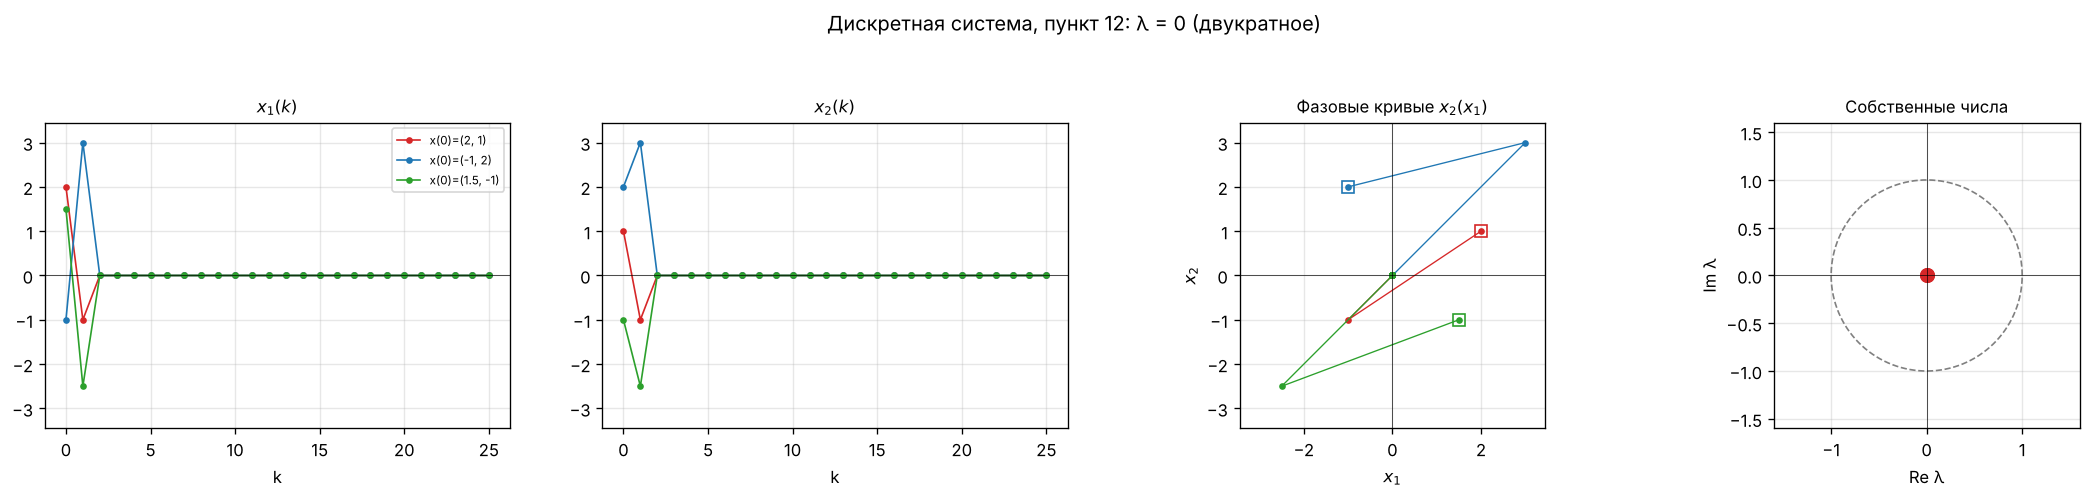
\includegraphics[width=\textwidth]{../graphics/d12_system.png}
        \caption{Пункт 12. Нильпотентная матрица: $x(k)=0$ при $k\ge2$}
        \label{fig:d12}
    \end{figure}

    \subsection{Закономерности}
    Поведение дискретной системы определяют положение собственных чисел относительно единичной окружности и их аргумент:
    \begin{itemize}
        \item $|\lambda|<1$ (внутри окружности) --- затухание, $|x(k)|\to0$; чем ближе к нулю, тем быстрее (пункты 6--8). $\lambda=0$ --- сходимость за конечное число шагов (пункт 12).
        \item $|\lambda|>1$ (вне окружности) --- рост (пункты 9--11), система неустойчива.
        \item $|\lambda|=1$ (на окружности) --- границы устойчивости: при диагонализуемой матрице траектории ограничены (пункты 2--4, система устойчива, не асимптотически); при жордановой клетке --- линейный рост (пункты 1 и 5), система неустойчива.
        \item Аргумент $\varphi=\arg\lambda$ определяет характер движения: $\varphi=0$ --- монотонное движение (пункты 5, 8, 11), $\varphi=\pi$ --- чередование знака (1, 6, 9), $0<\varphi<\pi$ --- колебания с поворотом на $\varphi$ за шаг и спираль (2, 3, 4, 7, 10); период колебаний $2\pi/\varphi$.
    \end{itemize}

    \section{Задание 3. Осциллятор}
    Система $\dot x_1=x_2$, $\dot x_2=ax_1+bx_2$ эквивалентна уравнению $\ddot x_1-b\dot x_1-ax_1=0$, матрица $A=\begin{pmatrix}0&1\\a&b\end{pmatrix}$, $\tr A=b$, $\det A=-a$. Характеристическое уравнение $\lambda^2-b\lambda-a=0$, $\lambda_{1,2}=\dfrac{b\pm\sqrt{b^2+4a}}2$; собственный вектор для $\lambda$ --- $(1,\lambda)^T$ (из первой строки $\lambda x_1=x_2$). Физический смысл переменных во всех примерах: $x_1$ --- координата (отклонение), $x_2=\dot x_1$ --- скорость; $a$ --- коэффициент возвращающей (при $a<0$) или выталкивающей (при $a>0$) силы, делённый на инерцию; $b$ --- коэффициент вязкого трения, делённый на инерцию (при $b<0$ трение).

    \textbf{Классификация по $a,b$:}
    \begin{itemize}
        \item $a<0$, $b=0$: $\lambda=\pm i\sqrt{|a|}$ --- центр, устойчиво (не асимптотически);
        \item $a<0$, $b<0$: $\mathrm{Re}\,\lambda=b/2<0$ --- устойчивый фокус при $b^2<4|a|$ (узел при $b^2\ge4|a|$), асимптотически устойчиво;
        \item $a>0$, $b=0$: $\lambda=\pm\sqrt a$ --- седло, неустойчиво;
        \item $a>0$, $b<0$: $\lambda_1\lambda_2=-a<0$ --- седло, неустойчиво (трение не стабилизирует).
    \end{itemize}

    \subsection{Случай 1. $a<0$, $b=0$}
    \textbf{Физическая система:} груз массы $m$ на пружине жёсткости $k$ без трения (или LC-контур). $x_1$ --- смещение от положения равновесия, $x_2$ --- скорость, $a=-k/m=-\omega_0^2$, $b=0$ (трения нет). Берём $a=-4$ ($k=4$ Н/м, $m=1$ кг, $\omega_0=2$ рад/с).
    $$A=\MatOA,\quad\lambda=\pm2i,\quad\text{собственные векторы }(1,\,\pm2i)^T.$$
    Обобщённых нет. Тип портрета --- \textbf{центр}: замкнутые эллипсы, незатухающие гармонические колебания $x_1(t)=C\cos(2t+\varphi)$ с периодом $\pi$; энергия сохраняется. Система устойчива, но не асимптотически. Начальные условия: $(1,0)^T$, $(0,2)^T$, $(-1.5,1)^T$, $(2,-1)^T$.
    \begin{figure}[H]
        \centering
        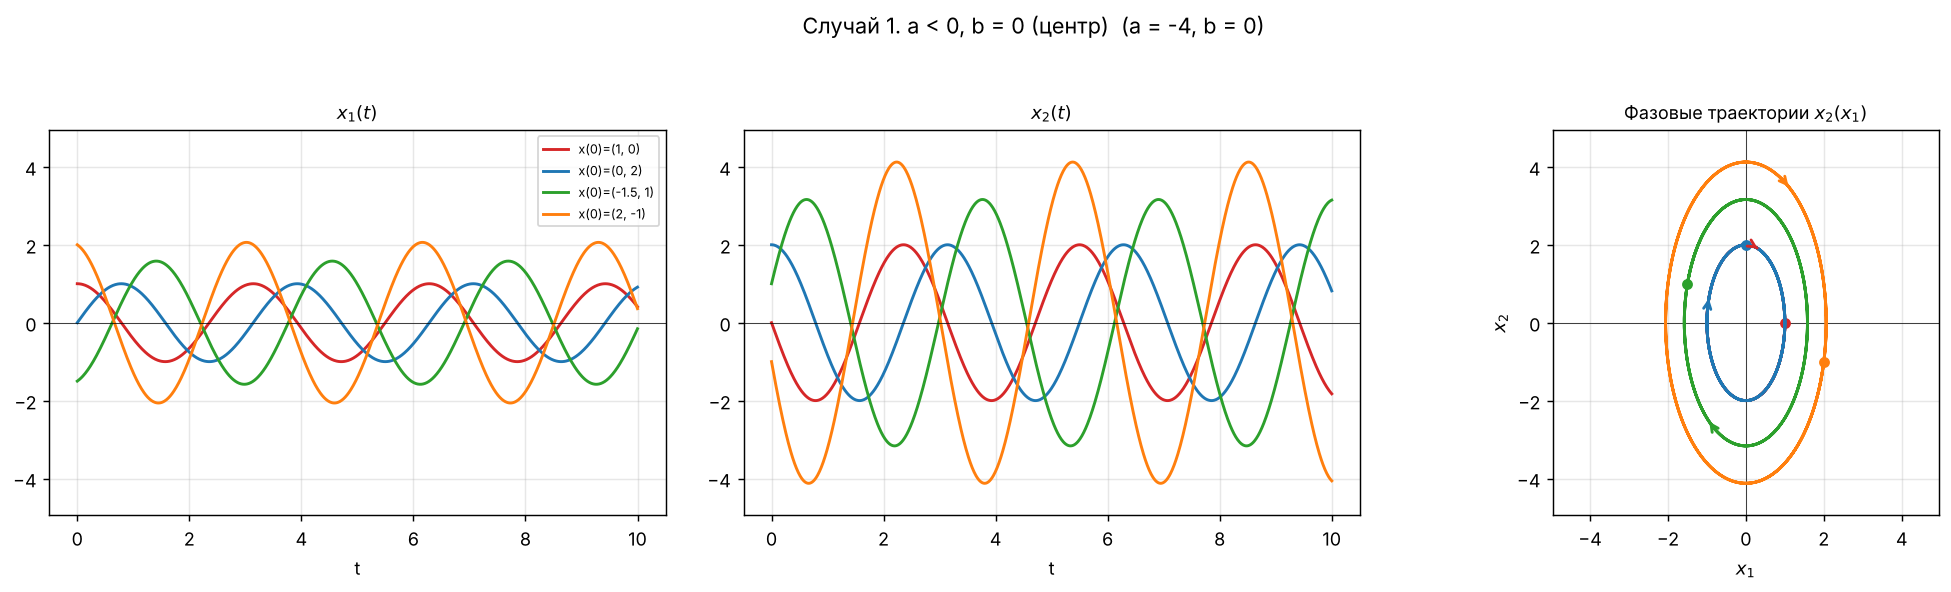
\includegraphics[width=\textwidth]{../graphics/o1_system.png}
        \caption{Случай 1. Незатухающие колебания (центр)}
        \label{fig:o1}
    \end{figure}

    \subsection{Случай 2. $a<0$, $b<0$}
    \textbf{Физическая система:} груз на пружине с вязким трением (или последовательный RLC-контур, где $x_1$ --- заряд, $x_2$ --- ток). $a=-k/m$, $b=-\gamma/m$, где $\gamma$ --- коэффициент вязкого трения. Берём $a=-4$, $b=-0.6$ ($\gamma=0.6$ Н$\cdot$с/м, $m=1$ кг): $b^2<4|a|$ (малое трение).
    $$A=\MatOB,\quad\lambda=-0.3\pm1.9774i,\quad\text{собств. векторы }(1,\,-0.3\pm1.9774i)^T.$$
    \textbf{Тип: устойчивый фокус.} Затухающие колебания с огибающей $e^{-0.3t}$ и частотой $\approx1.98$ рад/с; траектории закручиваются к началу, система асимптотически устойчива.
    \begin{figure}[H]
        \centering
        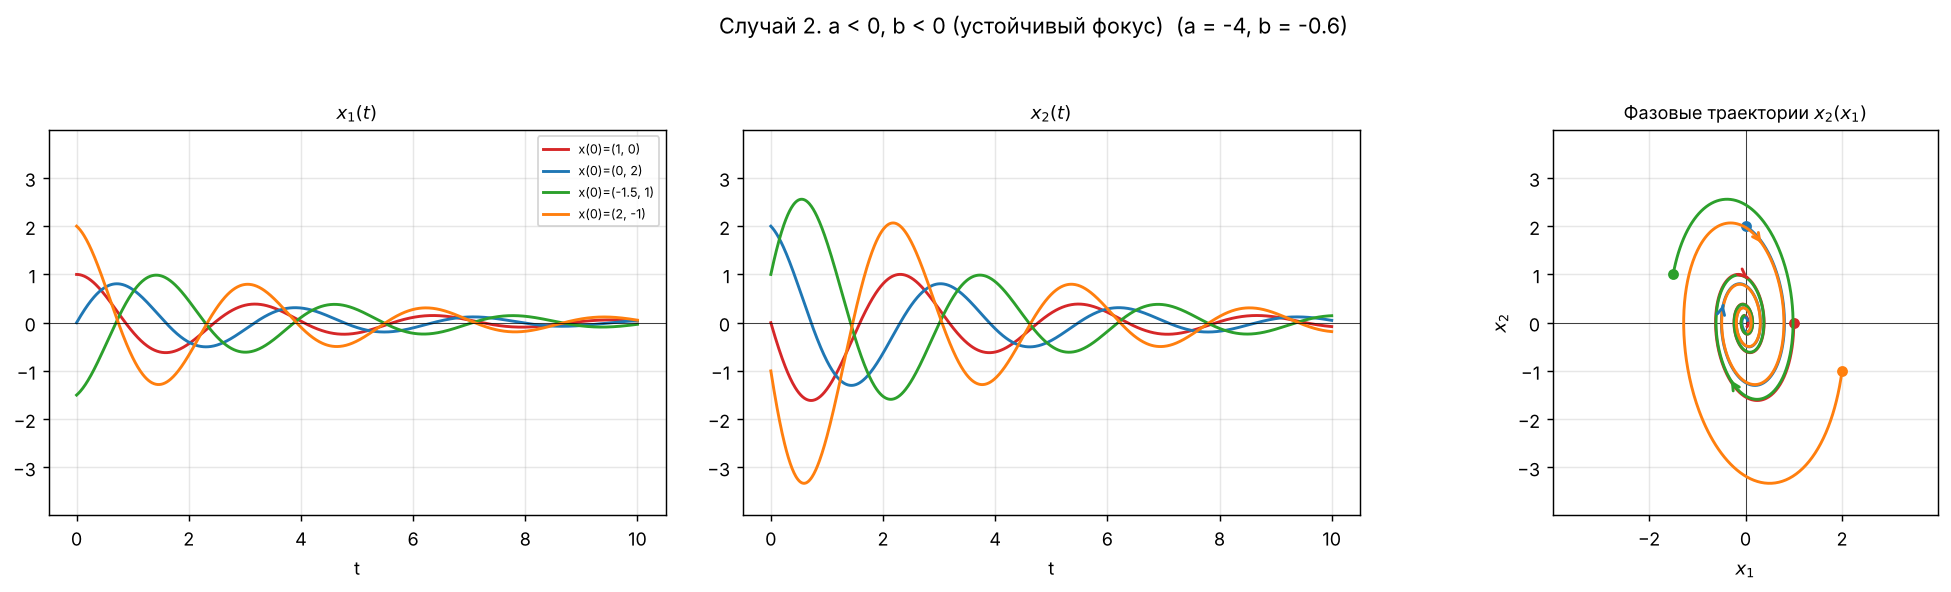
\includegraphics[width=\textwidth]{../graphics/o2_system.png}
        \caption{Случай 2. Затухающие колебания (устойчивый фокус)}
        \label{fig:o2}
    \end{figure}

    \subsection{Случай 3. $a>0$, $b=0$}
    \textbf{Физическая система:} перевёрнутый маятник в верхнем положении без трения (линеаризация вблизи вертикали) или шарик на вершине гладкой горки. $x_1$ --- отклонение угла от вертикали, $x_2$ --- угловая скорость, $a=g/l$, $b=0$. Берём $a=4$ с$^{-2}$ ($l\approx2.45$ м).
    $$A=\MatOC,\quad\lambda=2,\ -2,\quad\text{векторы }(1,\,2)^T,\ (1,\,-2)^T.$$
    \textbf{Тип: седло.} Неустойчиво: $x(t)=c_1e^{2t}(1,2)^T+c_2e^{-2t}(1,-2)^T$, отклонение растёт экспоненциально. Устойчивые траектории --- только при $x(0)\in\Span\{(1,-2)^T\}$ (маятник «заброшен» к вертикали с точно подобранной скоростью), на рисунке~\ref{fig:o3s}.
    \begin{figure}[H]
        \centering
        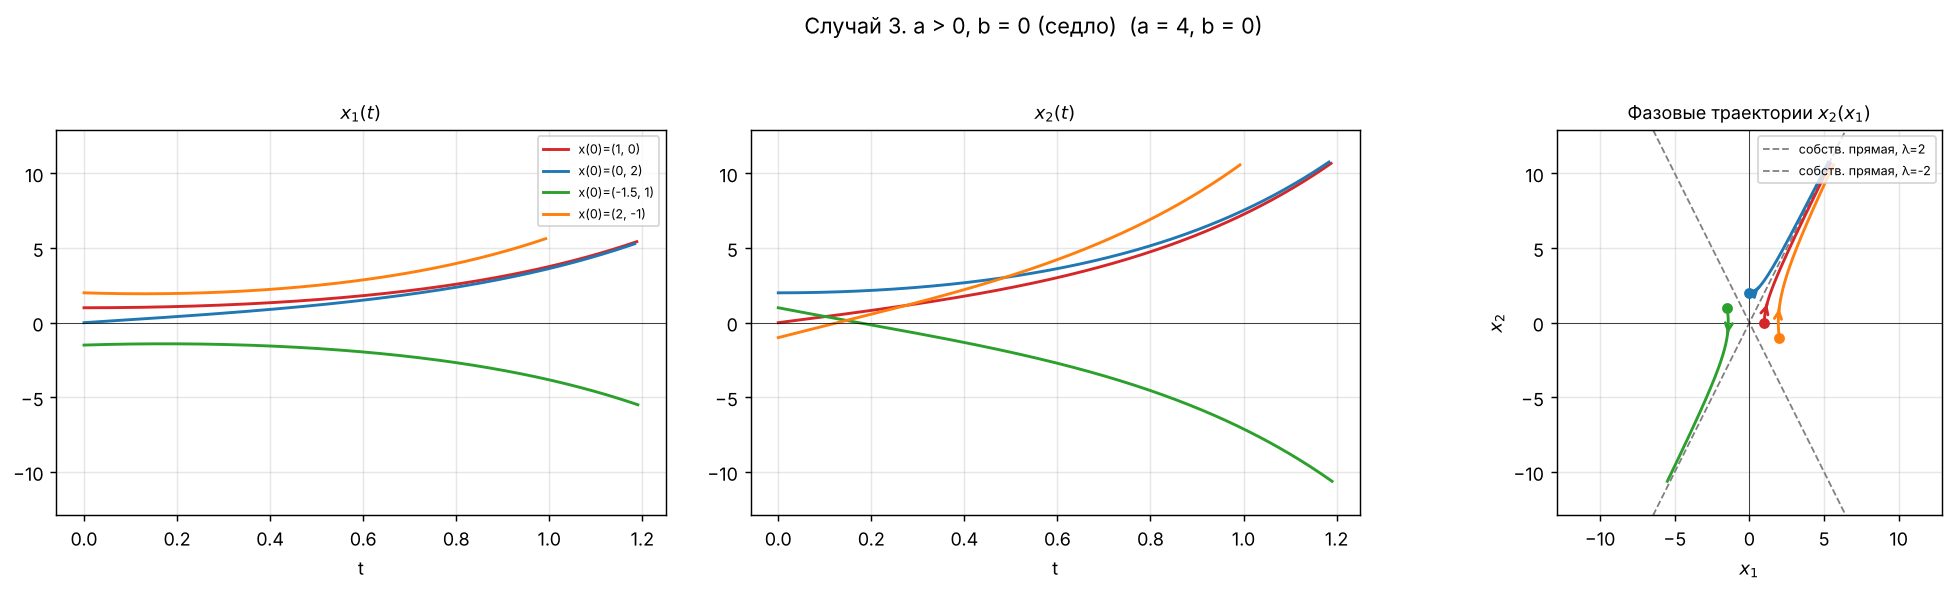
\includegraphics[width=\textwidth]{../graphics/o3_system.png}
        \caption{Случай 3. Седло, экспоненциальное удаление от положения равновесия}
        \label{fig:o3}
    \end{figure}
    \begin{figure}[H]
        \centering
        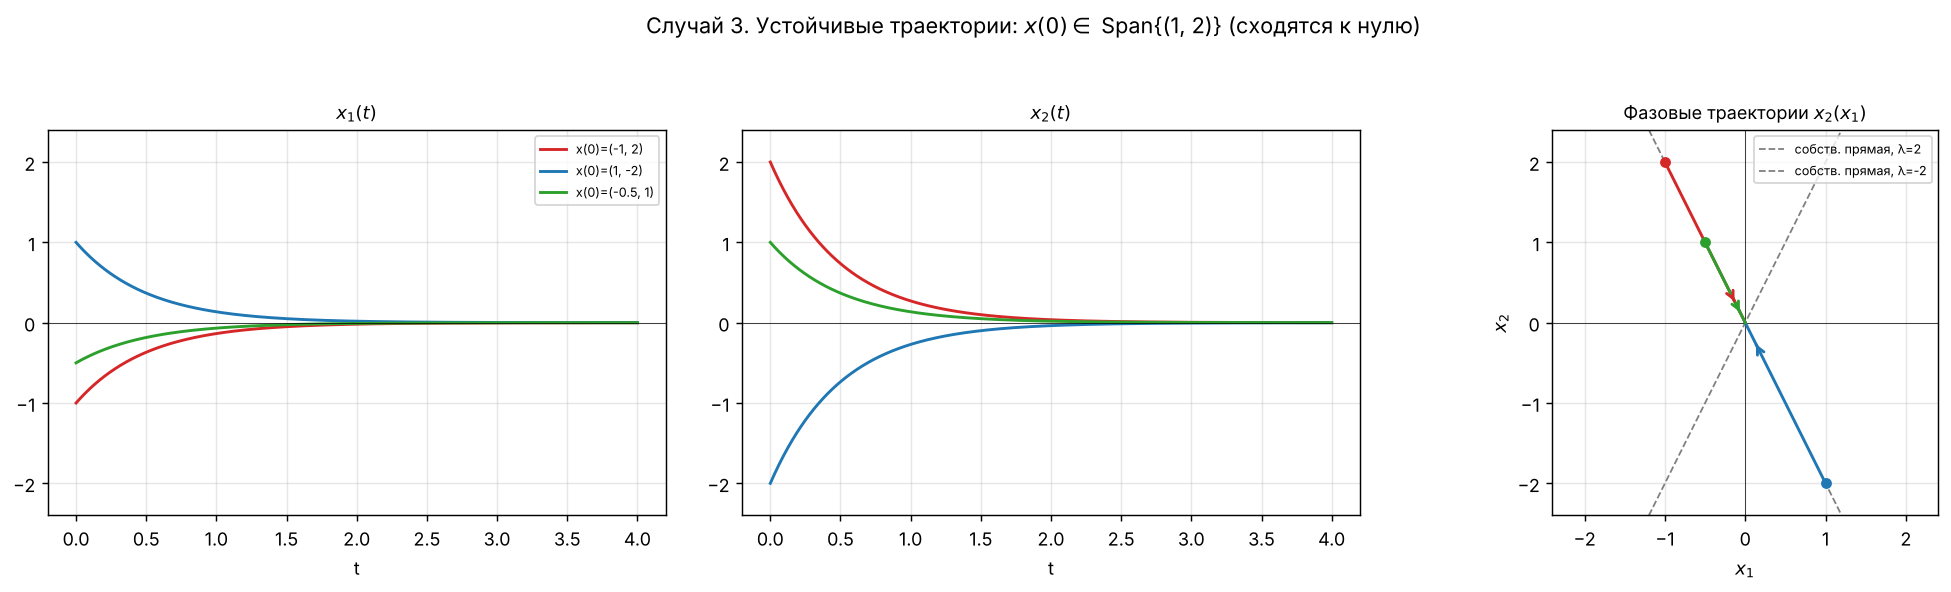
\includegraphics[width=\textwidth]{../graphics/o3_stable_only.png}
        \caption{Случай 3. Устойчивые траектории: $x(0)\in\Span\{(1,-2)^T\}$}
        \label{fig:o3s}
    \end{figure}

    \subsection{Случай 4. $a>0$, $b<0$}
    \textbf{Физическая система:} перевёрнутый маятник с вязким трением в оси (или шарик на горке в вязкой среде). $a=g/l>0$, $b=-\gamma/(ml^2)<0$. Берём $a=4$, $b=-1$.
    $$A=\MatOD,\quad\lambda=1.5616,\ -2.5616,\quad\text{векторы }(1,\,1.5616)^T,\ (1,\,-2.5616)^T.$$
    \textbf{Тип: седло.} Трение уменьшает скорость роста, но не стабилизирует положение равновесия: $\det A=-a<0$ при любом $b$. Устойчивые траектории --- только на $\Span\{(1,-2.5616)^T\}$ (рисунок~\ref{fig:o4s}).
    \begin{figure}[H]
        \centering
        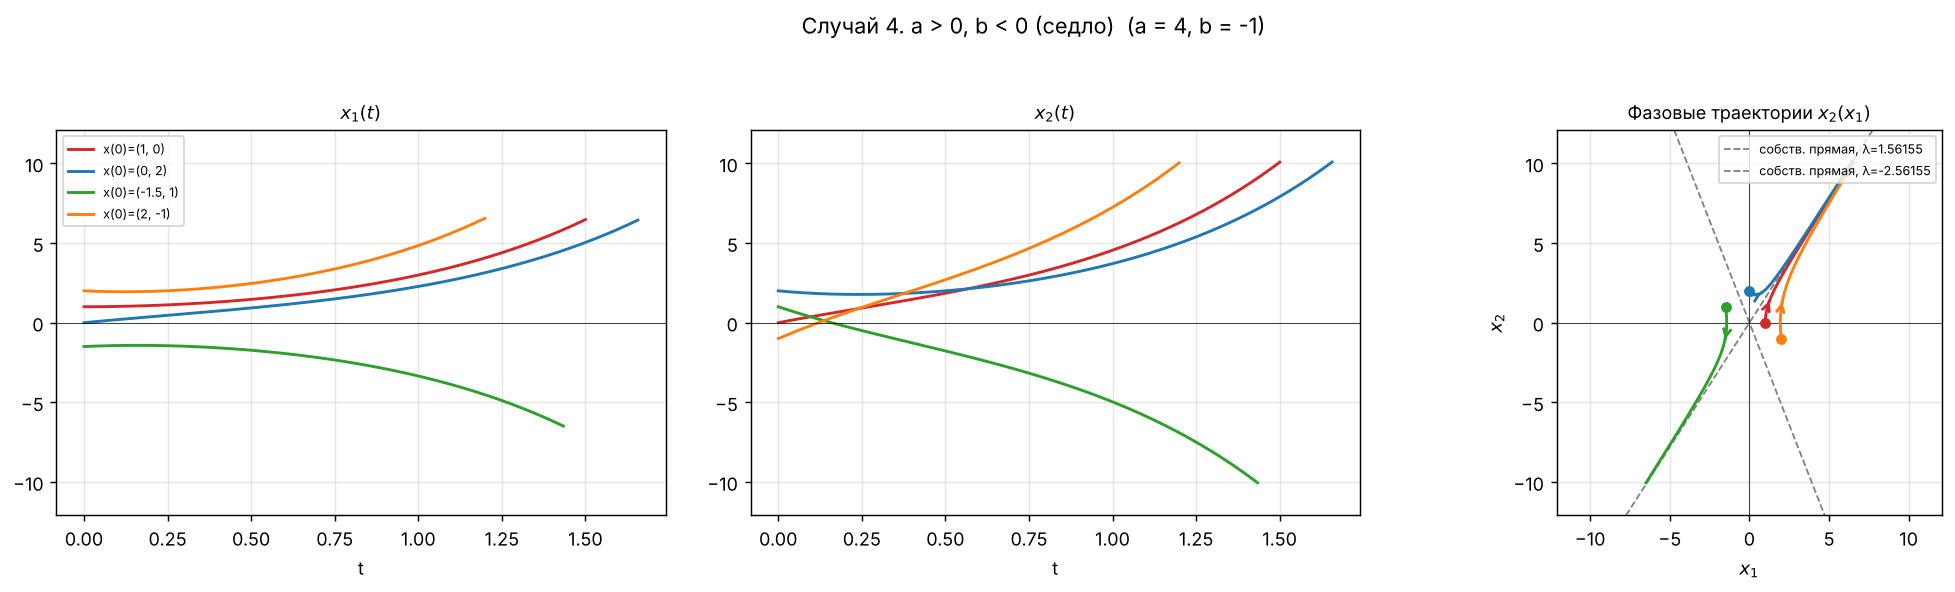
\includegraphics[width=\textwidth]{../graphics/o4_system.png}
        \caption{Случай 4. Седло с трением}
        \label{fig:o4}
    \end{figure}
    \begin{figure}[H]
        \centering
        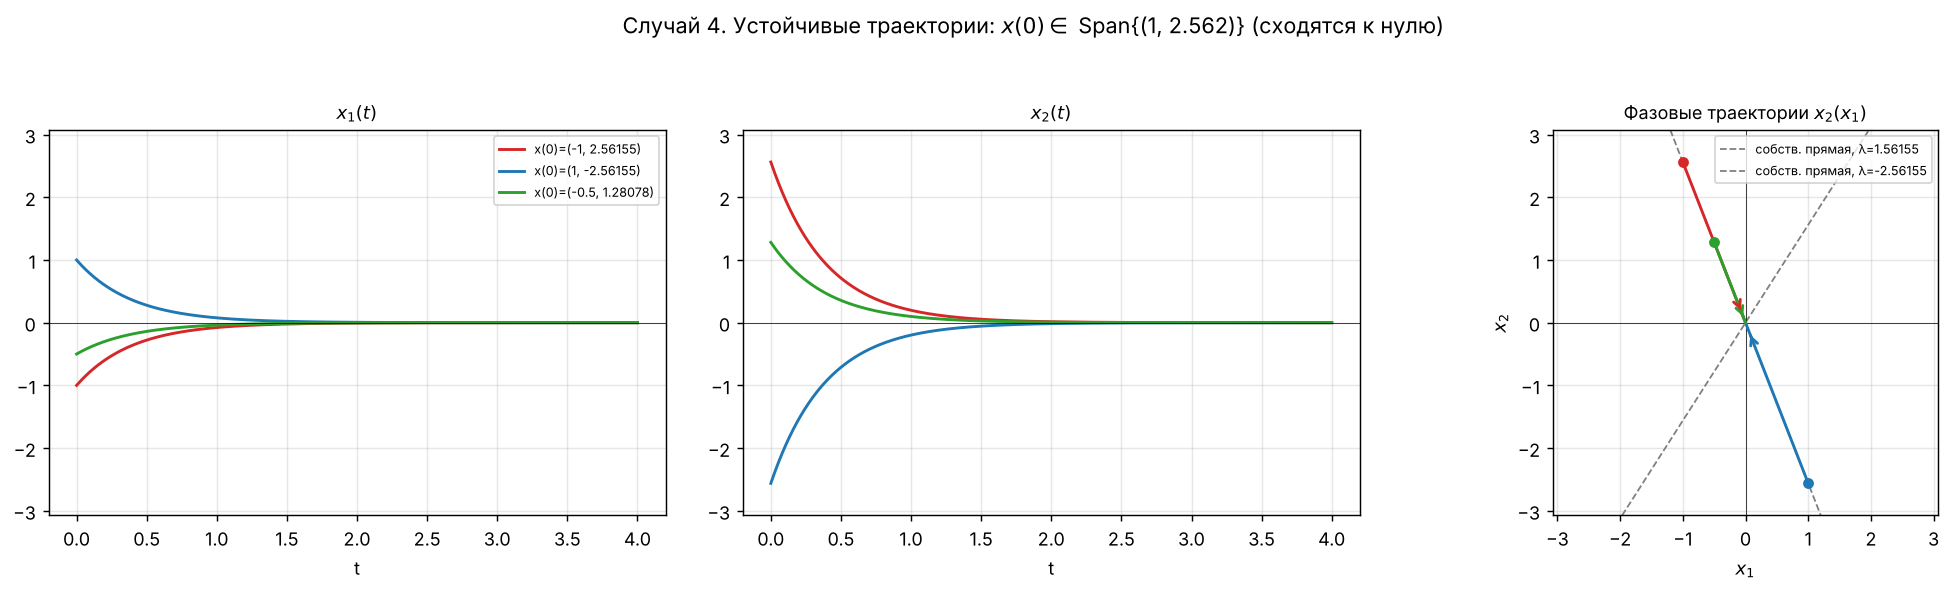
\includegraphics[width=\textwidth]{../graphics/o4_stable_only.png}
        \caption{Случай 4. Устойчивые траектории: $x(0)\in\Span\{(1,-2.5616)^T\}$}
        \label{fig:o4s}
    \end{figure}

    \section{Выводы}
    Для линейных систем $\dot x=Ax$ и $x(k+1)=Ax(k)$ тип движения и устойчивость определяются собственными числами матрицы, а направления инвариантных прямых --- её собственными векторами. В непрерывном случае граница устойчивости --- мнимая ось ($\mathrm{Re}\,\lambda=0$), в дискретном --- единичная окружность ($|\lambda|=1$); на границе устойчивость зависит от жордановой структуры (наличие клетки размера~2 делает систему неустойчивой). Построены системы с узлом, вырожденным узлом, седлом, фокусами и центром; проверено, что комплексные собственные векторы $v_1\pm iv_2$ дают вращательное движение в базисе $(v_1,v_2)$, знак $\mathrm{Re}\,\lambda$ определяет его затухание или рост. В дискретном случае аргумент собственного числа задаёт угол поворота за шаг, модуль --- множитель роста; нильпотентная матрица ($\lambda=0$) обнуляет состояние за конечное число шагов. Для осциллятора $\dot x_1=x_2$, $\dot x_2=ax_1+bx_2$ знак $a$ определяет, колебательное это движение ($a<0$) или седло ($a>0$), а знак $b$ --- затухают ли колебания (трение). Все матрицы и свойства проверены в программе численно (\texttt{assert}).

    \section{Приложение. Код выполнения}
\lstinputlisting[caption={Программа моделирования и построения графиков}, label={lst:code}]{../prog/main.py}

\end{document}
